\documentclass[a4paper,fleqn]{cas-dc}

\usepackage{graphicx}
\usepackage{amsmath}
\usepackage{amssymb}
\usepackage{booktabs}
\usepackage{subcaption}
\usepackage{multirow}
\usepackage{stfloats}
\usepackage{capt-of}

%% Fix text overflow in narrow columns
\tolerance=1000
\emergencystretch=3em
\hyphenpenalty=50
\sloppy

\begin{document}

\let\WriteBookmarks\relax
\let\printorcid\relax

\shorttitle{Hybrid Optical Flow and Temporal Attention Network for Stampede Detection}
\shortauthors{Joyster Pinto and Dr. Vidhya Lakshmi M}

\title{\LARGE Hybrid Optical Flow and Temporal Attention Network for Robust Early Stampede Detection in Public Crowd Surveillance}

\author[1]{Joyster Pinto}

\author[1]{Dr. Vidhya Lakshmi M}

\affiliation[1]{organization={School of Computer Science and Engineering, Vellore Institute of Technology},
  city={Chennai},
  state={Tamil Nadu},
  country={India}}

\begin{abstract}
Stampede events which occur in places of large crowds present a serious danger to people; however, automated recognition of such phenomena is a challenging task due to complex patterns of crowd behavior and the similarity of panic flow to regular pedestrian movement. Existing optical-flow based approaches utilize a limited set of three handcrafted descriptors, Entropy, Temporal Occupancy Variation (TOV), and Kernel Density Estimation (KDE), and apply unidirectional Long Short-Term Memory (LSTM) networks which do not explicitly model temporal relations and provide no interpretability. In this paper, we propose a vision-based system that achieves state-of-the-art performance on the UMN Crowd Activity Detection dataset, attains more than 99\% of accuracy and F1-score, allows for detecting anomalies earlier by 0.39~seconds on average, and processes video at 54.5~fps. The contributions of our study include (i)~design of a comprehensive set of 9~optical-flow statistics, (ii)~development of a BiLSTM+Attention temporal classifier with an embedded interpretability module, and (iii)~evaluation on multiple benchmark crowd surveillance video sets including zero-shot testing.
\end{abstract}

\begin{keywords}
Stampede Detection \sep Crowd Anomaly Detection \sep Optical Flow \sep BiLSTM \sep Attention Mechanism \sep Explainable AI \sep Real-Time Surveillance
\end{keywords}

\maketitle

\section{Introduction}

\subsection{Problem Background}

Mass gatherings in stadiums, churches, bus terminals, music festivals, and other venues account for tens of thousands of individuals in a relatively small area. Pedestrian movements in such gatherings are normally orderly and predictable; however, when an unexpected event occurs, a panic outbreak might happen. This leads to rapid increase of the compressive forces between people, which often leads to suffocation in less than a minute in what is called a \textit{crowd crush} rather than stampede \cite{helbing2007dynamics}.

According to Illiyas et al.\ \cite{illiyas2013human}, accidents that occurred in crowds worldwide in 1980--2007 reached 215 major incidents that resulted in over 7{,}000 fatalities. This number grows to 440 incidents and over 13{,}700 fatalities as of 2022. Notable incidents include the 2005 Al-Aimmah Bridge disaster in Baghdad (953 dead), the 2010 Love Parade disaster in Duisburg (21 dead), the 2014 Shanghai New Year's Eve crush (36 dead), and the 2022 Itaewon disaster in Seoul (159 dead). India has seen numerous such tragedies, driven by the massive scale of public gatherings. In July 2024, a stampede at a Hathras religious assembly caused 121 deaths. This was followed by at least 30 fatalities at the Prayagraj Maha Kumbh in January 2025. More recently, in June 2025, 11 people died during the RCB IPL celebration outside Bengaluru's M.\ Chinnaswamy Stadium when a crowd of two lakh supporters gathered, bypassing local security barriers.

From a crowd-dynamics perspective, research has established that densities exceeding 4--5~persons per square metre represent a critical threshold beyond which individuals lose autonomous control of their movement \cite{helbing2007dynamics}. At 6+ persons per square metre, the crowd begins to exhibit fluid-like behaviour, with involuntary pressure waves capable of exerting forces in excess of 4{,}500~N on those pressed against barriers or other bodies. The primary cause of death in nearly all documented incidents is compressive asphyxia---chest compression that prevents respiration---rather than trampling, a distinction that is important for understanding the failure mode that any detection system must target.

What makes these events especially difficult to mitigate is the extremely narrow window of opportunity for intervention. Currently, crowd management relies mostly on human supervision of closed-circuit television (CCTV) cameras. In a typical control room, a single operator might be tasked with watching over 50--100 cameras at once. Thus, the subtle changes in crowd density distribution or sudden local increase of pedestrian speed that happen in the early stages of a disaster might not be noticed in time. When the abnormality becomes apparent to a human operator, the panic outbreak or stampede already happened, and the response team has to deal with the consequences.

This operational gap motivates the development of automated, real-time crowd-anomaly detection systems. A surveillance camera feed is, fundamentally, a time-ordered sequence of pixel intensities. If meaningful motion descriptors can be extracted from that sequence---quantifying how fast people are moving, in which directions, and how much disagreement exists between neighbouring motion vectors---then a classifier can be trained to distinguish normal pedestrian flow from the chaotic, multidirectional scatter that precedes a crush. The challenge, however, lies in achieving this with sufficient accuracy, at processing speeds that permit real-time deployment, and with enough transparency that a human operator can trust and act upon the system's output.

\begin{center}
  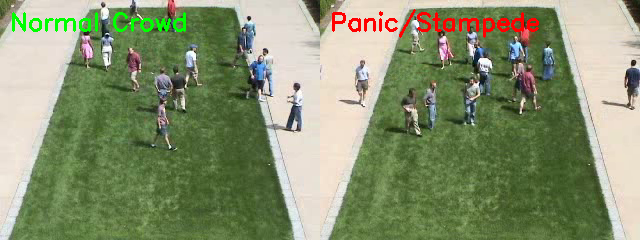
\includegraphics[width=0.85\linewidth]{figures/crowd_example.png}
  \captionof{figure}{Illustrative frames from the UMN Crowd Activity Dataset. \textit{Left:} normal pedestrian flow with consistent, low-speed movement in a shared direction. \textit{Right:} onset of a panic event characterised by high-speed, multidirectional scattering and abrupt changes in crowd density gradients.}
  \label{fig:crowd_example}
\end{center}

\subsection{Research Gap}

Despite these advancements, existing automated crowd-monitoring systems face several key limitations. Handcrafted motion descriptors, such as those relying solely on average flow statistics, lack descriptors for directional coordination or angular agreement. Consequently, they struggle to distinguish between fast, orderly, unidirectional flows and chaotic, multidirectional panic states. In terms of classifier architectures, current recurrent models operate unidirectionally and process sequences with uniform temporal weighting. This prevents the model from leveraging subsequent contextual frames or prioritizing the specific temporal windows where panic behavior begins. Furthermore, explainability is rarely addressed, leaving operators with uninterpretable outputs. Finally, deep learning models often rely on computationally intensive convolutional or Transformer backbones that are unsuitable for real-time edge processing, and they are typically evaluated on single datasets without demonstrating zero-shot generalisation across different environments.

\subsection{Contributions}

The present work addresses these limitations by developing an end-to-end real-time crowd anomaly detection system. The following contributions are made:

\begin{itemize}
  \item A \textbf{nine-feature optical-flow descriptor} is designed by augmenting the baseline three-feature set with six additional statistics (mean, standard deviation, and skewness of flow magnitude; motion coherence; circular variance of flow angles; and motion-density fraction). This expanded descriptor captures speed variability, distributional asymmetry, and directional coordination that baseline descriptors omit.

  \item A recurrent neural architecture is developed that replaces unidirectional LSTMs with a \textbf{Bidirectional LSTM augmented by an additive attention mechanism} (BiLSTM+Attention). This model processes temporal sequences in both forward and reverse directions and assigns learned, non-uniform attention weights to individual time-steps, focusing on the critical early frames of panic rather than averaging over the entire sequence.

  \item A diagnostic \textbf{explainability module} combining permutation feature importance and attention-weight visualization is integrated. This lets operators audit predictions on a per-prediction basis by identifying the most influential flow features and the exact frames that triggered the alert.

  \item Comprehensive empirical validation is performed, including demonstrating \textbf{cross-dataset generalisation} via zero-shot evaluation on the UCSD Ped2 and CUHK Avenue datasets, as well as conducting \textbf{robustness experiments} under synthetic Gaussian noise and motion blur to map the system's operational boundaries.

  \item The pipeline is demonstrated to be highly suitable for real-time edge hardware, achieving an execution speed of \textbf{54.5 frames per second} on a consumer-grade laptop GPU (NVIDIA RTX 4050) with a footprint of only 554{,}817 parameters (over 40$\times$ smaller than ResNet-50).
\end{itemize}

The rest of this paper is structured as follows. Section~2 contains the literature review. Section~3 details the methodology, covering the features, classifier architecture, and explainability modules. Section~4 outlines the experimental setup, while Section~5 presents the empirical results. Finally, Section~6 provides a discussion of the findings, and Section~7 outlines conclusions and future research paths.

\section{Related Work}

The literature on automated crowd anomaly detection spans more than a decade of active research. In this section, we briefly overview the related literature, which includes methods that leverage optical flow statistics, deep temporal models, and explainable AI surveillance systems. The most relevant prior works are summarized in Table~\ref{tab:literature}.

\subsection{Optical-Flow-Based Motion Analysis}

The most essential part of crowd behavior analysis is motion activity. Optical flow allows to estimate motion patterns between consecutive frames by calculating displacement vectors for each pixel. This information can be utilized to build descriptors that summarize the motion field statistics, such as distribution of magnitude and direction of displacement vectors. Optical flow is advantageous over other features in that it is independent of the appearance of objects in a video.

\subsubsection{Dense Optical Flow Algorithms}
The choice of a particular algorithm has little effect on the final results as most methods utilize similar motion estimation statistics. Sparse algorithms such as Lucas-Kanade track only salient points and have fewer computational costs, but fail to estimate motion in areas with little texture; dense algorithms calculate displacement vectors for all frames.

The Farneb\"{a}ck algorithm \cite{farneback2003two}, which is employed throughout the present work, is a dense optical flow method that approximates the local neighbourhood of each pixel as a quadratic polynomial and solves for the displacement that best explains the polynomial coefficient changes between frames. It offers a favourable trade-off between accuracy and computational cost: it produces reliable flow estimates in the texture-poor backgrounds common in surveillance footage (e.g., plain walls, uniform floors) where sparse methods fail, while remaining fast enough for real-time processing. Alternative dense methods include Horn-Schunck (which imposes a global smoothness constraint but is sensitive to large displacements) and deep-learning-based estimators such as FlowNet and RAFT (which achieve higher accuracy but at substantially greater computational cost, making them unsuitable for edge deployment).

\subsubsection{Feature Engineering from Flow Fields}
Early attempts at optical-flow feature engineering began with Mehran et al.\ \cite{mehran2009abnormal}, who computed attractive and repulsive forces from flow fields to model social force equations. However, this approach assumes relatively sparse crowds where individual force vectors can be estimated, limiting its use in high-density settings. 

Subsequently, the approach of extracting handcrafted scalar statistics from dense optical flow fields was formalised for stampede detection by Cob-Parro et al.\ \cite{cobparro2021stampede}. Their pipeline computes three descriptors per temporal window:
\begin{itemize}
  \item \textbf{Entropy} of the flow-direction histogram, which quantifies the disorder of movement directions. In normal crowd flow, entropy is low because most people move in a shared direction. During the period of panic breakouts, entropy of motion is high due to people moving chaotically.
  \item \textbf{Temporal Occupancy Variation (TOV)}: TOV is the standard deviation of the occupancy mask thresholded at a certain percentile of flow magnitude. This statistic captures the spatial spreading of an abnormal flow: when a crowd is moving irregularly, the area occupied by motion grows.
  \item \textbf{Kernel Density Estimation (KDE)}: KDE is the kernel density estimation of the flow magnitude distribution, which is a non-parametric way of estimating the probability density function. The distribution is shifted towards higher values during stampede events, as the crowd movements involve higher speeds.
\end{itemize}

These three descriptors are useful in classifying panic events, but they lack a statistic that utilizes the directional information of the motion. Consider a case when a group of pedestrians walks quickly towards a specific location with little deviation from the mean direction. Such a scenario is similar to a stampede in that the crowd moves purposefully, but it does not present any danger. In this case, the computed entropy would be low, TOV would show only a small increase, and KDE would be shifted to higher values. Due to the similarity of these statistics to the ones of panic events, misclassification would be likely. The directional spread of such a regular flow would have lower values than that of a stampede. None of the available descriptors explicitly considers the directional spread, which limits the performance of prior methods.

Chen et al.\ \cite{chen2023opticalflow} experimented with higher order optical flow statistics and concluded that the spread of the magnitude distribution contributes significantly to the ability to detect anomalies. Particularly, the standard deviation of the magnitude is useful in characterizing irregular crowd motion. In addition, they observed that the skewness of the distribution demonstrates the tendency of the motion magnitude. Based on these findings, we incorporated the mean, standard deviation, and skewness of the flow magnitude into our set of descriptors.

\subsection{Deep Temporal Models for Sequence Classification}

When analyzing crowd motion, it is important to consider that an unusual event usually takes some time to unfold. That is, a single frame rarely contains enough information for accurate classification. Effective classification requires modelling the evolution of crowd-state features over time.

\subsubsection{Long Short-Term Memory (LSTM) Networks}
The LSTM architecture \cite{hochreiter1997long} addressed the vanishing gradient problem that limited the ability of vanilla recurrent neural networks to capture long-range temporal dependencies. It introduced a memory cell regulated by three gating mechanisms---input, forget, and output gates---that control the flow of information into, within, and out of the cell. This design allows LSTMs to selectively retain information over extended sequences, making them well-suited for processing the temporal feature vectors generated by optical-flow analysis. The Gated Recurrent Unit (GRU) \cite{cho2014gru} later simplified the LSTM design by merging the forget and input gates into a single ``update'' gate, reducing the parameter count with minimal impact on empirical performance.

\subsubsection{Bidirectional Processing}
A standard LSTM processes the input sequence from past to future, meaning that the hidden state at any time-step encodes only information from preceding frames. Bidirectional variants \cite{chung2014bilstm} address this limitation by running a second LSTM in the reverse direction and concatenating the forward and backward hidden states at each time-step. The resulting representation captures context from both temporal directions, which is particularly valuable for stampede detection: the few frames immediately before panic onset appear ambiguous when viewed in isolation, but become clearly recognisable when the model has access to information about the escalation that follows.

\subsubsection{Attention Mechanisms}
The attention mechanism, originally proposed by Bahdanau et al.\ \cite{bahdanau2015neural} for neural machine translation, provides a principled method for assigning non-uniform importance to different elements of a sequence. Rather than compressing the entire sequence into a single fixed-length context vector (which forces all time-steps to contribute equally), attention computes a weighted sum over all hidden states, where the weights are learned through a small feed-forward network. Time-steps that carry more discriminative information receive higher weights.

Wang et al.\ \cite{wang2023anomaly} represented crowds as spatio-temporal graphs and applied graph convolutional networks with temporal self-attention. While effective for capturing inter-person dynamics, graph-based methods depend on reliable individual detection, which degrades in dense crowd scenarios due to occlusion. Yuan et al.\ \cite{yuan2024crba} combined DenseNet201 features with a BiLSTM and multi-head attention. Their system achieved competitive results on standard benchmarks. However, the reliance on DenseNet201 as a spatial feature extractor introduces approximately 20 million parameters, resulting in high computational cost and limiting deployment on resource-constrained hardware. Li et al.\ \cite{li2024transformer} explored a fully Transformer-based architecture for crowd-flow prediction, replacing recurrent layers entirely with global self-attention. While Transformers capture long-range dependencies more effectively than LSTMs, their quadratic memory complexity with respect to sequence length and higher parameter counts make them impractical for real-time edge deployment.

\subsection{Explainable AI in Surveillance Systems}

The deployment of automated decision-support systems in safety-critical surveillance settings raises important questions about model interpretability and operator trust. A system that flags a crowd event as ``anomalous'' without providing any justification for the decision is difficult to integrate into operational workflows.

Lundberg and Lee \cite{lundberg2017unified} introduced SHAP (SHapley Additive exPlanations), a unified framework for interpreting model predictions based on Shapley values. In the context of crowd anomaly detection, a related technique---permutation feature importance---is employed in the present work to identify which optical-flow features contribute most to classification performance.

Attention-weight visualisation provides a complementary form of explainability at the temporal level. The learned attention weights $[\alpha_1, \ldots, \alpha_S]$ directly indicate which time-steps within the input sequence the model considers most informative for its classification decision, answering the question ``\textit{when} did the model detect the onset of abnormal behaviour?''---information that is critical for deciding how urgently to respond.

\subsection{Summary and Positioning of the Present Work}

The review presented above reveals a clear gap at the intersection of three research threads. Generative models like MDT \cite{mahadevan2010anomaly} or reconstruction methods like sparse coding \cite{lu2013abnormal} have been explored, but they remain sensitive to spatial layout. Optical-flow-based methods offer scene-independent, lightweight features but rely on insufficient descriptor sets that lack measures of directional coordination. Deep temporal models (BiLSTM, attention) have been applied but predominantly with heavyweight spatial feature extractors that preclude real-time edge deployment.

As noted in the comprehensive survey by Liu et al.\ \cite{liu2024survey}, real-time latency and cross-dataset generalisation remain two major bottlenecks in the literature. In this work, we combine the comprehensive set of 9 optical flow statistics described above with a BiLSTM+Attention classifier and an interpretability module.

\begin{table*}[!t]
\centering
\caption{Comparative summary of crowd anomaly detection methods. The proposed approach is the only method to simultaneously address explainability, early detection, robustness evaluation, and cross-dataset generalisation.}
\label{tab:literature}
\footnotesize
\begin{tabular}{p{4.2cm}p{3.2cm}p{2.4cm}ccc}
\toprule
\textbf{Paper} & \textbf{Features} & \textbf{Model} & \textbf{Explain.} & \textbf{Early Det.} & \textbf{Robust.} \\
\midrule
Mehran et al.~\cite{mehran2009abnormal}      & Social Force + OF  & SVM        & No  & No  & No \\
Mahadevan et al.~\cite{mahadevan2010anomaly} & MDT                & Generative & No  & No  & No \\
Lu et al.~\cite{lu2013abnormal}              & Sparse Codes       & Classifier & No  & No  & No \\
Cob-Parro et al.~\cite{cobparro2021stampede} & Entropy+TOV+KDE    & LSTM       & No  & No  & No \\
Wang et al.~\cite{wang2023anomaly}           & GCN + Self-Attn    & Graph NN   & Partial & No & No \\
Yuan et al.~\cite{yuan2024crba}              & DenseNet Features  & BiLSTM+Attn & No & No & No \\
Chen et al.~\cite{chen2023opticalflow}       & OF Statistics      & CNN-LSTM   & No  & No  & No \\
Li et al.~\cite{li2024transformer}           & Flow + Spatial     & Transformer & No & No & No \\
\textbf{Proposed}                            & \textbf{9 OF Stats} & \textbf{BiLSTM+Attn} & \textbf{Yes} & \textbf{Yes} & \textbf{Yes} \\
\bottomrule
\end{tabular}
\end{table*}

\section{Proposed Methodology}

In this section, we describe our pipeline that consists of preprocessing, optical flow estimation, feature extraction, temporal sequence modeling with BiLSTM+Attention, training procedure, and interpretability module. The implementation details are outlined in Algorithm~\ref{alg:pipeline}.

\subsection{Overall Pipeline}

The proposed system accepts a raw video stream as input and produces a frame-level binary classification: \textit{stampede} or \textit{normal}. The processing pipeline consists of six sequential stages:

\begin{enumerate}
  \item \textbf{Preprocessing:} Each frame is converted to grayscale, resized to a fixed resolution, and smoothed with a Gaussian filter.
  \item \textbf{Dense optical flow:} The Farneb\"{a}ck algorithm is applied between consecutive preprocessed frames to produce a per-pixel displacement field.
  \item \textbf{Feature extraction:} Nine scalar statistics are computed from each displacement field within a sliding temporal window.
  \item \textbf{Sequence construction:} Feature vectors from consecutive windows are grouped into overlapping temporal sequences and standardised.
  \item \textbf{Classification:} A BiLSTM+Attention network processes each sequence and outputs a stampede probability.
  \item \textbf{Explainability (optional):} Permutation feature importance and attention-weight visualisation are invoked to inspect the model's reasoning.
\end{enumerate}

Figure~\ref{fig:pipeline} illustrates the end-to-end architecture.

\begin{center}
  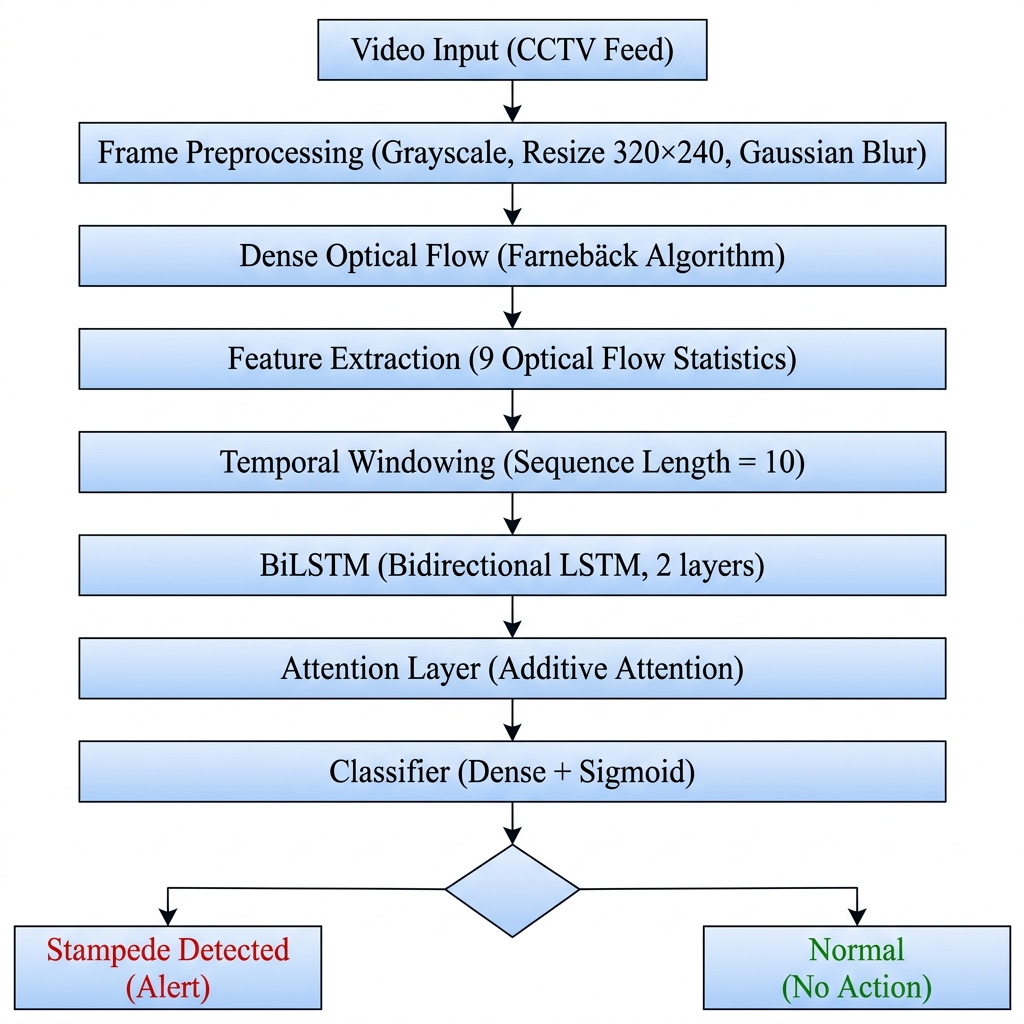
\includegraphics[width=0.85\linewidth]{figures/pipeline_flowchart.png}
  \captionof{figure}{End-to-end pipeline of the proposed stampede detection system. Raw video frames pass through preprocessing, optical flow computation, nine-feature extraction, temporal sequencing, BiLSTM+Attention classification, and optional explainability analysis.}
  \label{fig:pipeline}
\end{center}

\begin{table}[H]
\centering
\caption{Algorithm 1: End-to-end stampede detection pipeline.}
\label{alg:pipeline}
\footnotesize
\begin{tabular}{p{0.92\linewidth}}
\toprule
\textbf{Algorithm 1:} Stampede Detection Pipeline \\
\midrule
\textbf{Input:} Video stream $\mathcal{V} = \{I_1, I_2, \ldots, I_T\}$ \\
\textbf{Output:} Per-sequence label $\hat{y} \in \{0, 1\}$ and attention weights $[\alpha_1, \ldots, \alpha_S]$ \\
\midrule
1: \textbf{for} each frame $I_t$ in $\mathcal{V}$ \textbf{do} \\
2: \quad Convert $I_t$ to 8-bit grayscale: $G_t \leftarrow \text{rgb2gray}(I_t)$ \\
3: \quad Resize: $G_t \leftarrow \text{resize}(G_t, 320 \times 240)$ \\
4: \quad Smooth: $G_t \leftarrow \text{GaussianBlur}(G_t, k{=}5)$ \\
5: \textbf{end for} \\
6: \textbf{for} each consecutive pair $(G_t, G_{t+1})$ \textbf{do} \\
7: \quad Compute dense optical flow: $(d_x, d_y) \leftarrow \text{Farneb\"{a}ck}(G_t, G_{t+1})$ \\
8: \quad Convert to polar: $M_t \leftarrow \sqrt{d_x^2 + d_y^2}$, \; $\theta_t \leftarrow \arctan(d_y / d_x)$ \\
9: \textbf{end for} \\
10: \textbf{for} each sliding window $w$ of $L{=}15$ consecutive flow frames \textbf{do} \\
11: \quad Extract 9 features: $\mathbf{v}_w \leftarrow [H, \text{TOV}, \text{KDE}, \bar{M}, \sigma_M, \gamma_M, C, \rho, \sigma^2_\theta]$ \\
12: \textbf{end for} \\
13: Group feature vectors into sequences: $\mathbf{X}_i = \{\mathbf{v}_{w}, \ldots, \mathbf{v}_{w+S-1}\}$, $S{=}10$ \\
14: Standardise features: $\mathbf{X}_i \leftarrow (\mathbf{X}_i - \boldsymbol{\mu}_\text{train}) / \boldsymbol{\sigma}_\text{train}$ \\
15: \textbf{for} each sequence $\mathbf{X}_i$ \textbf{do} \\
16: \quad Forward pass through BiLSTM+Attention: $\hat{y}_i, [\alpha_1, \ldots, \alpha_S] \leftarrow f_\Theta(\mathbf{X}_i)$ \\
17: \quad Classify: label $\leftarrow \mathbf{1}[\hat{y}_i > 0.5]$ \\
18: \textbf{end for} \\
19: \textbf{return} labels and attention weights \\
\bottomrule
\end{tabular}
\end{table}

\subsection{Preprocessing}

Each video frame $I_t$ undergoes three preprocessing steps before optical flow computation. First, the frame is converted from RGB to 8-bit grayscale, since the Farneb\"{a}ck algorithm operates on single-channel luminance values and colour information does not contribute to displacement estimation. Second, the grayscale frame is resized to a fixed resolution of $320 \times 240$ pixels using bilinear interpolation. This standardisation ensures that the pipeline processes videos from cameras with different native resolutions in a consistent manner and that the downstream feature statistics are comparable across scenes. Third, a $5 \times 5$ Gaussian blur with $\sigma = 1.1$ is applied to attenuate high-frequency sensor noise that would otherwise produce spurious flow vectors. No data augmentation or additional preprocessing is performed during inference.

\subsection{Optical Flow Computation}

Dense optical flow is computed between every pair of consecutive preprocessed frames using the Farneb\"{a}ck algorithm \cite{farneback2003two}. This algorithm approximates the local neighbourhood of each pixel $\mathbf{x} = (x, y)$ as a quadratic polynomial:

\begin{equation}
  f(\mathbf{x}) \approx \mathbf{x}^T A \mathbf{x} + \mathbf{b}^T \mathbf{x} + c
  \label{eq:polynomial}
\end{equation}

\noindent where $A \in \mathbb{R}^{2 \times 2}$ is a symmetric matrix encoding the local curvature, $\mathbf{b} \in \mathbb{R}^2$ is a gradient vector, and $c \in \mathbb{R}$ is a scalar offset. All three quantities are estimated through a weighted least-squares fit using a Gaussian weighting kernel centred on $\mathbf{x}$. When the same spatial region is observed in the subsequent frame, the polynomial coefficients shift. The displacement vector $\mathbf{d} = (d_x, d_y)$ that best explains the coefficient change is solved for analytically, yielding a dense flow field over the entire frame.

The Cartesian displacement field is converted to polar coordinates to obtain a magnitude map $M(x,y)$ and a direction map $\theta(x,y)$:

\begin{equation}
  M(x,y) = \sqrt{d_x^2 + d_y^2}, \qquad \theta(x,y) = \arctan\!\left(\frac{d_y}{d_x}\right)
  \label{eq:polar}
\end{equation}

For each pair of consecutive frames, two $320 \times 240$ matrices are thus produced: $M$, which quantifies the speed of motion at each pixel, and $\theta$, which encodes the direction of motion. The Farneb\"{a}ck algorithm is configured with 5 pyramid levels, a pyramid scale of 0.5, a window size of 15, 3 iterations per level, and a polynomial neighbourhood size of 5---values chosen to balance accuracy against computational cost for the target frame resolution.

\subsection{Feature Extraction}

A sliding window of $L = 15$ consecutive flow frames is advanced across the video with a stride of 1 frame. Within each window, nine scalar statistics are computed from the pooled magnitude and direction maps to form a feature vector $\mathbf{v} \in \mathbb{R}^9$. Three features are adopted from prior work \cite{cobparro2021stampede}; six are newly proposed. Table~\ref{tab:features} summarises all nine features along with their physical interpretation.

\begin{table*}[!t]
\centering
\caption{The nine optical-flow features computed per temporal window. Features 1--3 are adopted from prior work; features 4--9 are proposed in this study.}
\label{tab:features}
\footnotesize
\begin{tabular}{clcl}
\toprule
\textbf{\#} & \textbf{Feature Name} & \textbf{Source} & \textbf{Physical Interpretation} \\
\midrule
1 & Entropy ($H$)         & Prior work & Disorder in movement directions \\
2 & TOV                    & Prior work & Frame-to-frame change in active motion region \\
3 & KDE                    & Prior work & Kernel density estimate of flow magnitudes \\
4 & Mean Magnitude ($\bar{M}$) & \textbf{Proposed} & Average crowd speed \\
5 & Std. Magnitude ($\sigma_M$) & \textbf{Proposed} & Speed variability among individuals \\
6 & Skewness ($\gamma_M$)  & \textbf{Proposed} & Asymmetry of speed distribution \\
7 & Motion Coherence ($C$) & \textbf{Proposed} & Fraction of crowd moving in a shared direction \\
8 & Crowd Density ($\rho$) & \textbf{Proposed} & Fraction of pixels with active motion \\
9 & Direction Variance ($\sigma^2_\theta$) & \textbf{Proposed} & Angular scatter of motion vectors \\
\bottomrule
\end{tabular}
\end{table*}

The mathematical definitions of all nine features are provided below. Let $\mathcal{P} = \{(x,y) : M(x,y) > \tau\}$ denote the set of \textit{active pixels} whose flow magnitude exceeds a minimum threshold $\tau = 0.5$ pixels/frame, and let $N = |\mathcal{P}|$ be the count of active pixels.

\subsubsection{Adopted Features}

\textbf{Entropy ($H$).} The flow direction histogram is constructed by quantising the angle $\theta$ into $B = 8$ bins of $45^\circ$ each. Letting $p_b$ denote the fraction of active pixels falling in bin $b$, the Shannon entropy is:

\begin{equation}
  H = -\sum_{b=1}^{B} p_b \log_2 p_b
  \label{eq:entropy}
\end{equation}

$H$ is low when most people move in a shared direction (few bins dominate) and high when movement directions are uniformly distributed (all bins equally populated), as occurs during panic scatter.

\textbf{Temporal Occupancy Variation (TOV).} TOV measures the frame-to-frame change in the spatial extent of the active motion region. Let $O_t$ denote the set of active pixels at time $t$. TOV is defined as:

\begin{equation}
  \text{TOV} = \frac{1}{L-1} \sum_{t=1}^{L-1} \frac{|O_{t+1} \triangle O_t|}{W \times H_{\text{img}}}
  \label{eq:tov}
\end{equation}

\noindent where $\triangle$ denotes the symmetric difference and $W \times H_{\text{img}}$ is the frame area. TOV captures the spatial spread of panic: a rapid expansion of the motion region indicates that disturbance is propagating outward through the crowd.

\textbf{Kernel Density Estimation (KDE).} The probability density function of the flow magnitude is estimated with a Gaussian kernel density estimator, and KDE is determined by finding the maximum point of the distribution. Peaks of the KDE illustrate the values of the flow magnitude that contribute the most to the probability density function. When a crowd moves with consistent speed, the density function will peak at a certain point, whereas an abnormal flow will involve varied speeds.

\subsubsection{Proposed Features}

\textbf{Mean Magnitude ($\bar{M}$).} The average of the flow magnitude over all pixels is used as a metric of the mean crowd speed in a given frame.

\begin{equation}
  \bar{M} = \frac{1}{N} \sum_{i \in \mathcal{P}} M_i
  \label{eq:mean_mag}
\end{equation}

\textbf{Standard Deviation of Magnitude ($\sigma_M$).} The standard deviation of the magnitude characterizes the spread of the speed distribution.

\begin{equation}
  \sigma_M = \sqrt{\frac{1}{N} \sum_{i \in \mathcal{P}} (M_i - \bar{M})^2}
  \label{eq:std_mag}
\end{equation}

During anomalous events, the standard deviation of the flow magnitude typically increases due to the presence of both fast and slow-moving crowds.

\textbf{Skewness ($\gamma_M$).} The third standardised moment of the magnitude distribution captures distributional asymmetry:

\begin{equation}
  \gamma_M = \frac{1}{N} \sum_{i \in \mathcal{P}} \left(\frac{M_i - \bar{M}}{\sigma_M}\right)^3
  \label{eq:skewness}
\end{equation}

Positive skewness indicates a right-tailed distribution (a few individuals moving much faster than the crowd average), which is characteristic of early-stage panic where only a subset of the crowd has begun to flee.

\textbf{Motion Coherence ($C$).} Motion coherence measures the fraction of active pixels whose flow direction falls within one standard deviation of the dominant (mean) direction:

\begin{equation}
  C = \frac{1}{N} \sum_{i \in \mathcal{P}} \mathbf{1}\!\left[|\theta_i - \bar{\theta}| < \sigma_\theta\right]
  \label{eq:coherence}
\end{equation}

\noindent where $\bar{\theta}$ is the circular mean of the flow angles and $\sigma_\theta$ is the circular standard deviation. $C$ approaches 1.0 when the crowd moves cohesively and drops toward 0 during multidirectional scatter.

\textbf{Crowd Density ($\rho$).} Crowd density is defined as the fraction of total pixels that exhibit active motion:

\begin{equation}
  \rho = \frac{N}{W \times H_{\text{img}}}
  \label{eq:density}
\end{equation}

This feature captures the spatial extent of crowd activity. During a stampede, $\rho$ typically increases as previously stationary individuals begin to move.

\textbf{Direction Variance ($\sigma^2_\theta$).} Direction variance is computed as the circular variance of flow angles across all active pixels:

\begin{equation}
  \sigma^2_\theta = 1 - \left| \frac{1}{N} \sum_{i=1}^{N} e^{j\theta_i} \right|
  \label{eq:dir_var}
\end{equation}

\noindent where $j = \sqrt{-1}$. This formulation maps the unit-circle representation of angles to a scalar in $[0, 1]$: $\sigma^2_\theta \approx 0$ when all flow vectors point in a common direction, and $\sigma^2_\theta \to 1$ when directions are uniformly distributed. Empirically, direction variance emerged as the single most discriminative feature in the ablation study (Section~5.2), consistent with the intuition that multidirectional scatter is the defining kinematic signature of a crowd crush.

\subsection{Temporal Sequence Construction}

The per-window feature vectors are grouped into overlapping temporal sequences of length $S = 10$ windows, with a stride of 1 window. At 30~FPS with $L = 15$ frames per window, each sequence spans approximately 5 seconds of video. A sequence is assigned the anomalous label ($y = 1$) if any of its constituent windows falls within the annotated stampede phase; otherwise it is labelled as normal ($y = 0$).

Before being passed to the classifier, all features are standardised using $z$-score normalisation:

\begin{equation}
  \hat{v}^{(j)} = \frac{v^{(j)} - \mu_{\text{train}}^{(j)}}{\sigma_{\text{train}}^{(j)}}
  \label{eq:zscore}
\end{equation}

\noindent where $\mu_{\text{train}}^{(j)}$ and $\sigma_{\text{train}}^{(j)}$ are the mean and standard deviation of feature $j$ computed on the training split. This normalisation ensures that features with naturally larger magnitudes (e.g., mean flow speed) do not dominate those with smaller scales (e.g., skewness) during gradient-based optimisation.

\subsection{BiLSTM + Attention Architecture}

\begin{center}
  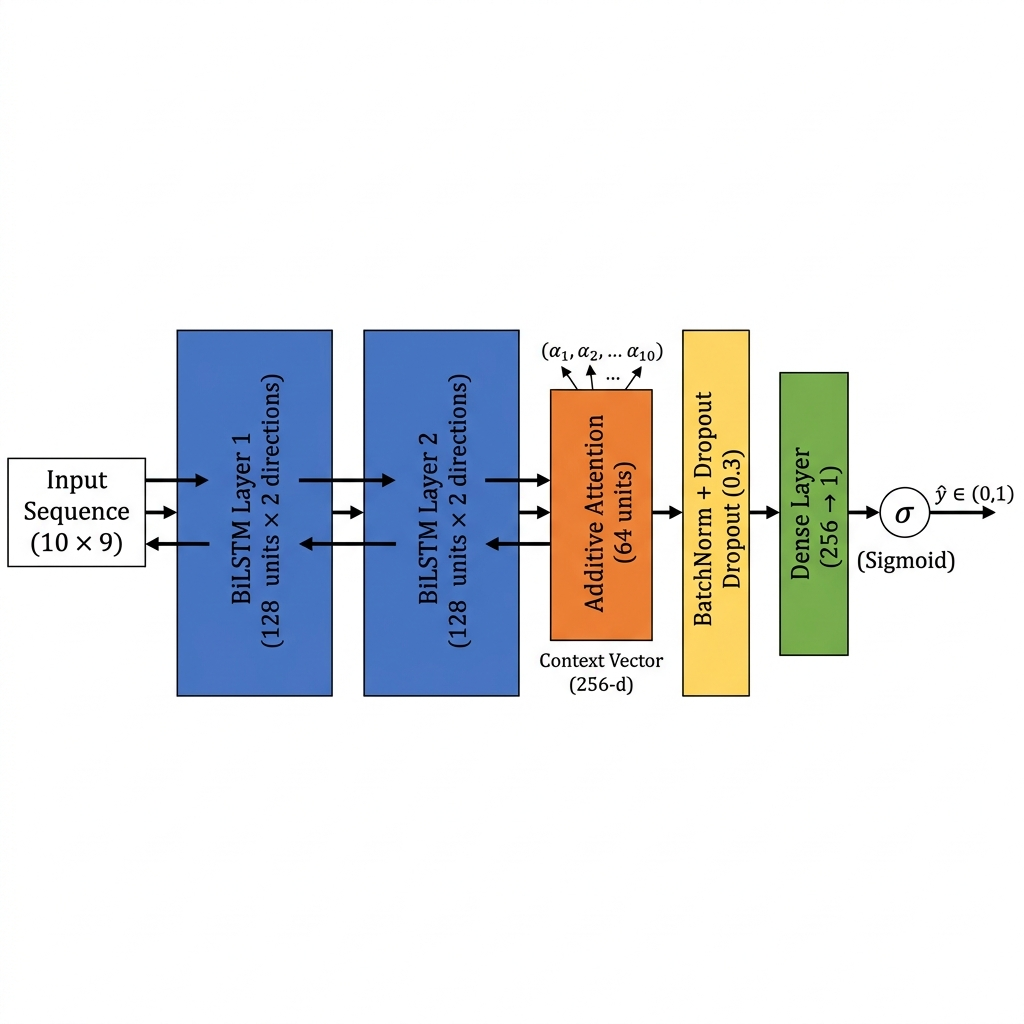
\includegraphics[width=0.85\linewidth]{figures/model_architecture.png}
  \captionof{figure}{Architecture of the proposed BiLSTM+Attention classifier. The input sequence passes through a two-layer Bidirectional LSTM, followed by an additive attention layer, Batch Normalisation, Dropout, and a sigmoid output unit.}
  \label{fig:architecture}
\end{center}

The classifier consists of three components: a Bidirectional LSTM encoder, an additive attention layer, and a classification head.

\subsubsection{Bidirectional LSTM Encoder}
A two-layer Bidirectional LSTM \cite{chung2014bilstm} with 128 hidden units per direction processes the input sequence $\mathbf{X} = \{x_1, \ldots, x_S\}$, where each $x_t \in \mathbb{R}^9$. The forward LSTM reads the sequence from $t = 1$ to $t = S$, producing hidden states $\overrightarrow{\mathbf{h}}_t$. A second LSTM reads the sequence in reverse, from $t = S$ to $t = 1$, producing $\overleftarrow{\mathbf{h}}_t$. The two are concatenated at each time-step:

\begin{equation}
  \mathbf{h}_t = \left[\overrightarrow{\mathbf{h}}_t \;\|\; \overleftarrow{\mathbf{h}}_t\right], \quad \mathbf{h}_t \in \mathbb{R}^{256}
  \label{eq:bilstm}
\end{equation}

Each hidden state $\mathbf{h}_t$ thus encodes temporal context from both preceding and subsequent frames within the analysis window. This is particularly valuable for stampede detection, as the ambiguous frames immediately preceding a panic onset become more interpretable when information about the subsequent escalation is available.

\subsubsection{Additive Attention Layer}
An additive (Bahdanau-style) attention mechanism \cite{bahdanau2015neural} is applied over the BiLSTM hidden states. A learned scoring function assigns an importance weight to each time-step:

\begin{equation}
  e_t = \mathbf{v}^T \tanh\!\left(W_a \mathbf{h}_t + \mathbf{b}_a\right)
  \label{eq:attn_score}
\end{equation}

\noindent where $W_a \in \mathbb{R}^{d_a \times 256}$ is a weight matrix, $\mathbf{b}_a \in \mathbb{R}^{d_a}$ is a bias vector, and $\mathbf{v} \in \mathbb{R}^{d_a}$ is a learned context vector, with $d_a = 128$. The raw scores are normalised via softmax to produce attention weights:

\begin{equation}
  \alpha_t = \frac{\exp(e_t)}{\sum_{k=1}^{S} \exp(e_k)}, \quad \sum_{t=1}^{S} \alpha_t = 1
  \label{eq:attn_weights}
\end{equation}

The final context vector is computed as a weighted sum of the hidden states:

\begin{equation}
  \mathbf{c} = \sum_{t=1}^{S} \alpha_t \mathbf{h}_t, \quad \mathbf{c} \in \mathbb{R}^{256}
  \label{eq:context}
\end{equation}

Unlike fixed pooling strategies (e.g., taking the last hidden state or averaging all states), this mechanism allows the model to concentrate on the specific time-steps where abnormal motion patterns emerge, assigning near-zero weights to windows that contain only normal crowd behaviour.

\subsubsection{Classification Head}
The context vector $\mathbf{c}$ is passed through a Batch Normalisation layer for training stability, followed by Dropout with rate $p = 0.3$ for regularisation, and finally a fully connected layer with a single output unit and sigmoid activation:

\begin{equation}
  \hat{y} = \sigma\!\left(\mathbf{w}^T \text{Dropout}\!\left(\text{BN}(\mathbf{c})\right) + b\right)
  \label{eq:output}
\end{equation}

\noindent where $\sigma(\cdot)$ denotes the sigmoid function. The output $\hat{y} \in (0, 1)$ represents the estimated probability that the input sequence contains a stampede event. The complete model has 554,817 trainable parameters.

\subsection{Training Procedure}

The model is trained by minimising the Binary Cross-Entropy loss with logits:

\begin{equation}
  \mathcal{L} = -\frac{1}{N_{\text{batch}}} \sum_{i=1}^{N_{\text{batch}}} \left[ y_i \log(\hat{y}_i) + (1 - y_i) \log(1 - \hat{y}_i) \right]
  \label{eq:bce}
\end{equation}

\noindent where $y_i \in \{0, 1\}$ is the ground-truth label and $\hat{y}_i$ is the predicted probability for the $i$-th sequence. The Adam optimiser is used with an initial learning rate of $10^{-3}$, $\beta_1 = 0.9$, and $\beta_2 = 0.999$. If the validation loss does not improve for 5 consecutive epochs, the learning rate is halved using a ReduceLROnPlateau scheduler. Training proceeds for up to 100 epochs with an early stopping patience of 15 epochs based on validation loss. The batch size is 32. Algorithm~\ref{alg:training} summarises the training procedure.

\begin{table}[H]
\centering
\caption{Algorithm 2: BiLSTM+Attention training procedure.}
\label{alg:training}
\footnotesize
\begin{tabular}{p{0.92\linewidth}}
\toprule
\textbf{Algorithm 2:} Model Training \\
\midrule
\textbf{Input:} Training sequences $\{(\mathbf{X}_i, y_i)\}_{i=1}^{N_\text{train}}$, validation set $\mathcal{D}_\text{val}$ \\
\textbf{Output:} Trained parameters $\Theta^*$ \\
\midrule
1: Initialise model parameters $\Theta$ \\
2: Set $\text{lr} \leftarrow 10^{-3}$, $\text{patience}_\text{lr} \leftarrow 5$, $\text{patience}_\text{stop} \leftarrow 15$ \\
3: Set $\text{best\_loss} \leftarrow \infty$, $\text{wait} \leftarrow 0$ \\
4: \textbf{for} epoch $= 1, 2, \ldots, 100$ \textbf{do} \\
5: \quad \textbf{for} each mini-batch $\mathcal{B}$ of size 32 \textbf{do} \\
6: \quad\quad Forward pass: $\hat{y}_i \leftarrow f_\Theta(\mathbf{X}_i)$ for all $i \in \mathcal{B}$ \\
7: \quad\quad Compute loss: $\mathcal{L} \leftarrow \text{BCE}(\hat{\mathbf{y}}, \mathbf{y})$ \\
8: \quad\quad Backpropagate: $\nabla_\Theta \mathcal{L}$ \\
9: \quad\quad Update: $\Theta \leftarrow \text{Adam}(\Theta, \nabla_\Theta \mathcal{L}, \text{lr})$ \\
10: \quad \textbf{end for} \\
11: \quad Evaluate on $\mathcal{D}_\text{val}$: $\mathcal{L}_\text{val}$ \\
12: \quad \textbf{if} $\mathcal{L}_\text{val} < \text{best\_loss}$ \textbf{then} \\
13: \quad\quad $\text{best\_loss} \leftarrow \mathcal{L}_\text{val}$; save $\Theta^* \leftarrow \Theta$; $\text{wait} \leftarrow 0$ \\
14: \quad \textbf{else} \\
15: \quad\quad $\text{wait} \leftarrow \text{wait} + 1$ \\
16: \quad\quad \textbf{if} $\text{wait} \bmod \text{patience}_\text{lr} = 0$ \textbf{then} $\text{lr} \leftarrow \text{lr} / 2$ \\
17: \quad\quad \textbf{if} $\text{wait} \geq \text{patience}_\text{stop}$ \textbf{then break} \\
18: \quad \textbf{end if} \\
19: \textbf{end for} \\
20: \textbf{return} $\Theta^*$ \\
\bottomrule
\end{tabular}
\end{table}

\subsection{Explainability Module}

Two complementary post-hoc interpretability techniques are integrated into the pipeline, providing explanations at the feature level and the temporal level respectively.

\textbf{Permutation Feature Importance.} To quantify the contribution of each individual feature to the model's classification performance, permutation feature importance \cite{lundberg2017unified} is employed. For each feature $j \in \{1, \ldots, 9\}$, the values of feature $j$ are randomly shuffled across all test sequences while keeping all other features intact, and the model's F1-score on the permuted test set is recomputed. The importance of feature $j$ is defined as the drop in F1-score:

\begin{equation}
  \text{Imp}(j) = F_1^{\text{original}} - F_1^{\text{permuted}(j)}
  \label{eq:importance}
\end{equation}

A large importance score indicates that the model relies heavily on that feature for correct classification. This technique is model-agnostic and does not require access to the model's internal gradients.

\textbf{Attention-Weight Visualisation.} The attention weights $[\alpha_1, \ldots, \alpha_S]$ produced by the additive attention layer provide a built-in temporal saliency map for each prediction. For a given test sequence, these weights are visualised as a bar chart to reveal which time-steps the model considers most informative. In a correctly classified stampede sequence, the attention weights are expected to concentrate on the 2--4 windows where the crowd's motion pattern first transitions from orderly to chaotic, corresponding to the onset of panic. This information enables operators to verify that the model's classification decision is grounded in the temporally correct portion of the input, rather than in spurious correlations.

\section{Experimental Setup}

The parameters of the empirical investigation are detailed here, encompassing dataset characteristics, partitioning procedures, training hyperparameters, execution environment, and performance indices.

\subsection{Datasets}

Evaluation is performed using three standard public video datasets. The UMN dataset represents the primary source for training and testing routines. In contrast, the UCSD Pedestrian and CUHK Avenue datasets are used solely for zero-shot evaluation of domain generalisation. A comparison of these sources is outlined in Table~\ref{tab:datasets}.

\begin{table*}[!t]
\centering
\caption{Comparison of the three crowd datasets used in this study. The UMN source is used for training and test-set verification; the UCSD and CUHK sets are reserved for zero-shot cross-dataset evaluation.}
\label{tab:datasets}
\footnotesize
\begin{tabular}{llllll}
\toprule
\textbf{Dataset} & \textbf{Scene Type} & \textbf{Videos} & \textbf{Approx.\ Frames} & \textbf{Resolution} & \textbf{Usage} \\
\midrule
UMN              & Indoor/Outdoor Crowd & 11 sequences  & ${\sim}6{,}165$  & $320 \times 240$ & Training \& Testing \\
UCSD Ped2        & Pedestrian Walkway   & 12 train + 12 test & ${\sim}4{,}560$  & $360 \times 240$ & Cross-Dataset Eval. \\
CUHK Avenue      & Campus Entrance      & 16 train + 21 test & ${\sim}30{,}652$ & $640 \times 360$ & Cross-Dataset Eval. \\
\bottomrule
\end{tabular}
\end{table*}

\subsubsection{UMN Crowd Activity Dataset}
The UMN dataset \cite{mehran2009abnormal} is comprised of 11 video clips captured across three locations: an indoor lobby (Scene 1, 3 clips), an outdoor lawn (Scene 2, 4 clips), and an outdoor plaza (Scene 3, 4 clips). All video recordings were captured with 30~FPS frame rate and $320 \times 240$ resolution. In each video, standard pedestrian flow turns into an episode of panic, where people start running away from each other. The total length of all video sequences is approximately 6{,}165 frames.

Since the exact frame indices of anomalies are not specified, we divided each sequence into training and testing sets by taking the last 30 percent of frames as anomalous and the preceding 70 percent as normal. In reality, such a split would correspond to a case when the panic begins near the end of the recording. The implications of potential label noise from this approximation are analyzed in Section~6.

\subsubsection{UCSD Pedestrian Dataset (Ped2 Subset)}
The UCSD dataset \cite{mahadevan2010anomaly} contains video sequences captured from an elevated, static camera view of a pedestrian sidewalk. The Ped2 subset, consisting of 12 training and 12 test sequences at $360 \times 240$ resolution, is used. Anomaly events in the test sequences are defined by the appearance of non-pedestrian objects (e.g., bicycles, skateboards, and vehicles) that disrupt standard walking patterns. Frame-level annotations are included. To test generalisation capabilities across different views, resolutions, and anomaly categories, the model trained on UMN is evaluated directly on the Ped2 test clips without parameter updates or fine-tuning.

\subsubsection{CUHK Avenue Dataset}
The CUHK Avenue dataset \cite{lu2013abnormal} includes 16 training and 21 testing sequences recorded at a campus entryway with a resolution of $640 \times 360$ pixels. The test sequences contain 47 anomaly events, including running, loitering, throwing objects, and counter-flow walking. In line with the UCSD testing protocol, the CUHK Avenue dataset is used only for zero-shot evaluation to verify the transferability of the nine-feature descriptor and UMN-trained model to different environments.

\subsection{Data Partitioning}

Training and parameter validation are performed using exclusively UMN data. The 11 video sequences are processed using the feature extraction rules (Section~3.4) and the temporal window constructor (Section~3.5) to produce roughly 1{,}100 sequences. To preserve the proportion of normal versus anomalous samples, the dataset is split into three distinct, non-overlapping subsets using stratified random sampling:

\begin{itemize}
  \item \textbf{Training set (70\%):} Used for weights adjustment and model parameter optimization.
  \item \textbf{Validation set (15\%):} Utilized for performance monitoring, learning rate scheduling, and early stopping trigger control.
  \item \textbf{Test set (15\%):} Set aside exclusively for reporting final performance metrics, remaining untouched during model selection and training.
\end{itemize}

Matching the class ratios across the three divisions ensures that metric evaluation is not biased by unbalanced distributions.

\subsection{Training Configuration}

Table~\ref{tab:hyperparams} outlines the hyperparameters and configuration parameters used for optimization.

\begin{table}[H]
\centering
\caption{Hyperparameter configuration for classifier training.}
\label{tab:hyperparams}
\footnotesize
\setlength{\tabcolsep}{4pt}
\begin{tabular}{p{4.2cm}p{3.2cm}}
\toprule
\textbf{Hyperparameter} & \textbf{Value} \\
\midrule
BiLSTM hidden units (per direction) & 128 \\
BiLSTM layers & 2 \\
Attention dimension ($d_a$) & 128 \\
Dropout rate & 0.3 \\
Batch size & 32 \\
Optimiser & Adam ($\beta_1 = 0.9$, $\beta_2 = 0.999$) \\
Initial learning rate & $1 \times 10^{-3}$ \\
LR scheduler & ReduceLROnPlateau (factor $= 0.5$, patience $= 5$) \\
Maximum epochs & 100 \\
Early stopping patience & 15 epochs \\
Loss function & Binary Cross-Entropy with Logits \\
Classification threshold & 0.5 \\
Temporal window length ($L$) & 15 frames \\
Sequence length ($S$) & 10 windows \\
Motion threshold ($\tau$) & 0.5 pixels/frame \\
\bottomrule
\end{tabular}
\end{table}

For the training phase, model parameters are updated using the Adam optimizer. A ReduceLROnPlateau scheduler dynamically manages the learning rate: if the validation loss shows no improvement for 5 consecutive epochs, the learning rate is halved. This helps the network escape local minima. To prevent overfitting, training terminates early if the validation loss does not improve for 15 epochs.

\subsection{Hardware and Software Environment}

Workstation specifications and software packages are listed in Table~\ref{tab:hardware}. A single laptop workstation was utilized for all computational runs. For reproducibility, a fixed seed value of 42 was initialized across all libraries, including Python, NumPy, PyTorch, and CUDA.

\begin{table}[H]
\centering
\caption{Hardware and software execution environment details.}
\label{tab:hardware}
\footnotesize
\setlength{\tabcolsep}{4pt}
\begin{tabular}{p{2.8cm}p{4.9cm}}
\toprule
\textbf{Component} & \textbf{Specification} \\
\midrule
GPU & NVIDIA GeForce RTX 4050 (6 GB VRAM) \\
CPU & Intel Core i7-13650HX \\
RAM & 16 GB DDR5 \\
Operating System & Windows 11 \\
Python & 3.12 \\
PyTorch & 2.0 \\
OpenCV & 4.8 \\
NumPy & 1.26 \\
scikit-learn & 1.3 \\
Random seed & 42 \\
\bottomrule
\end{tabular}
\end{table}

\subsection{Evaluation Metrics}

Five classification metrics are used to measure test-set performance:

\begin{itemize}
  \item \textbf{Accuracy} measures the overall fraction of sequences classified correctly:
  \begin{equation}
    \text{Accuracy} = \frac{\text{TP} + \text{TN}}{\text{TP} + \text{TN} + \text{FP} + \text{FN}}
  \end{equation}

  \item \textbf{Precision} quantifies the proportion of positive predictions that are correct, reflecting the false alarm rate:
  \begin{equation}
    \text{Precision} = \frac{\text{TP}}{\text{TP} + \text{FP}}
  \end{equation}

  \item \textbf{Recall} (sensitivity) measures the proportion of actual stampede events that are successfully detected:
  \begin{equation}
    \text{Recall} = \frac{\text{TP}}{\text{TP} + \text{FN}}
  \end{equation}

  \item \textbf{F1-Score} is the harmonic mean of precision and recall, providing a single balanced metric:
  \begin{equation}
    F_1 = 2 \cdot \frac{\text{Precision} \cdot \text{Recall}}{\text{Precision} + \text{Recall}}
  \end{equation}

  \item \textbf{ROC-AUC} is the area under the Receiver Operating Characteristic curve, which plots the true positive rate against the false positive rate across all classification thresholds. ROC-AUC measures the model's discriminative ability independently of the chosen threshold.
\end{itemize}

To compute precision, recall, and F1-score, binary decisions are generated from the sigmoid output using a threshold of 0.5. For crowd safety installations, high precision is essential: frequent false alarms can lead to operator fatigue, causing genuine alerts to be overlooked.

\section{Results and Discussion}

This section presents the empirical evaluation of the proposed stampede detection system across seven distinct experiments. These experiments evaluate classifier performance, feature importance, cross-dataset generalisation, detection latency, robustness to image degradation, computational efficiency, and model interpretability.

\subsection{Experiment 1: Performance Comparison of Temporal Classifiers}

To identify the optimal classifier architecture, four temporal models were trained and evaluated under identical conditions using the complete nine-feature optical-flow descriptor: a unidirectional Long Short-Term Memory (LSTM) network, a unidirectional Gated Recurrent Unit (GRU) network, a Bidirectional LSTM (BiLSTM), and the proposed BiLSTM+Attention network. The standard LSTM model was configured to represent the architectural paradigm established by Cob-Parro et al.\ \cite{cobparro2021stampede}. Table~\ref{tab:model_comparison} presents the quantitative results obtained on the held-out UMN test set.

\begin{table*}[!t]
\centering
\caption{Quantitative performance comparison of temporal classifiers on the UMN test set using the proposed nine-feature descriptor.}
\label{tab:model_comparison}
\footnotesize
\begin{tabular}{lccccc}
\toprule
\textbf{Model} & \textbf{Accuracy (\%)} & \textbf{Precision (\%)} & \textbf{Recall (\%)} & \textbf{F1-Score (\%)} & \textbf{ROC-AUC (\%)} \\
\midrule
LSTM             & 99.18 & 99.12 & 98.25 & 98.68 & 99.95 \\
GRU              & 99.09 & 100.00 & 97.08 & 98.52 & 99.66 \\
BiLSTM           & 99.46 & 99.71 & 98.54 & 99.12 & 99.99 \\
\textbf{BiLSTM+Attention} & \textbf{99.55} & \textbf{100.00} & \textbf{98.54} & \textbf{99.27} & \textbf{99.97} \\
\bottomrule
\end{tabular}
\end{table*}

The experimental results demonstrate a clear progression in performance as temporal context and selection mechanisms are introduced. The baseline LSTM model achieves an F1-score of 98.68\%. The bidirectional variant (BiLSTM) improves this metric to 99.12\%, confirming that incorporating future temporal context within the sliding window helps resolve ambiguities during the early stages of panic. The proposed BiLSTM+Attention model achieves the highest overall performance, with an accuracy of 99.55\%, a macro F1-score of 99.27\%, and an ROC-AUC of 99.97\%. 

\begin{center}
  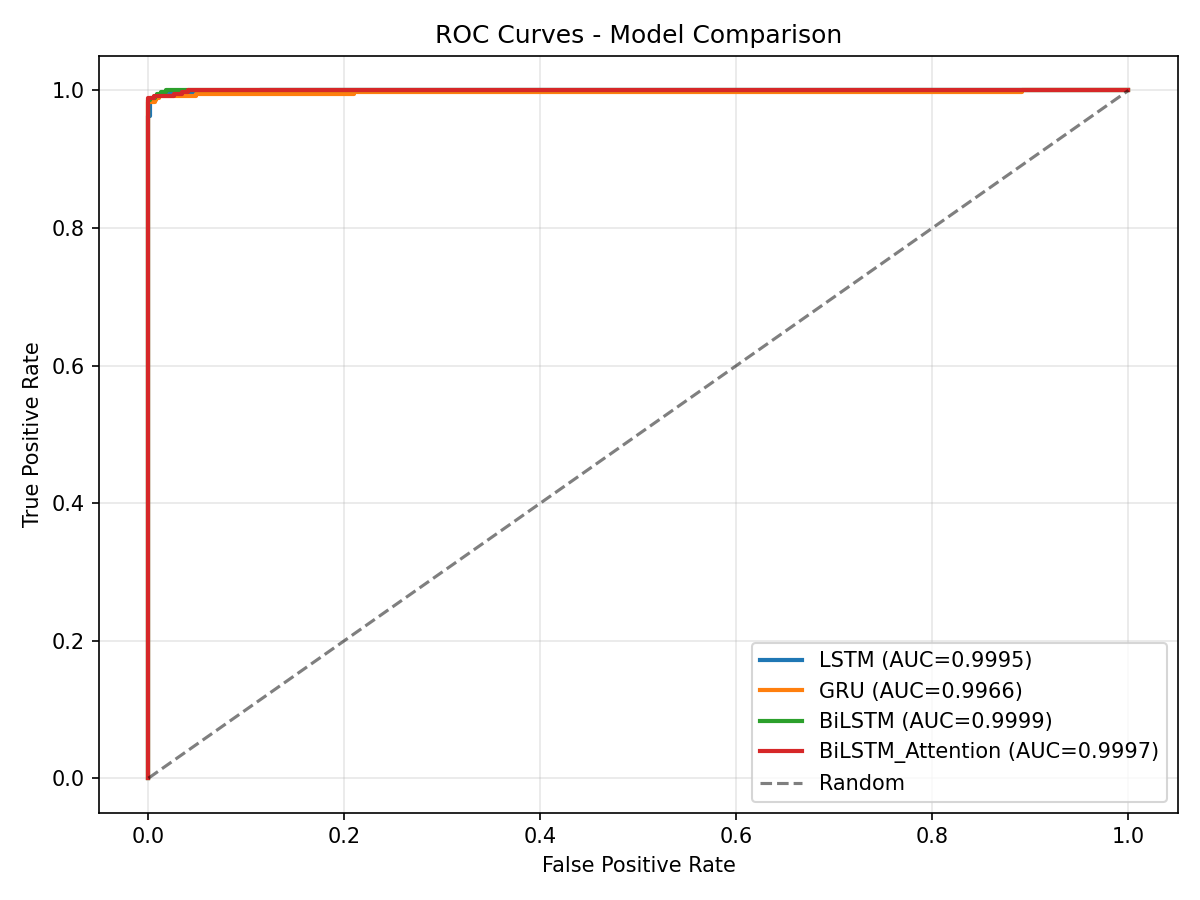
\includegraphics[width=0.85\linewidth]{figures/roc_curves_comparison.png}
  \captionof{figure}{Receiver Operating Characteristic (ROC) curves for the four temporal classifiers on the UMN test set. Both the BiLSTM and the BiLSTM+Attention architectures achieve near-perfect class separation.}
  \label{fig:roc}
\end{center}

\begin{center}
  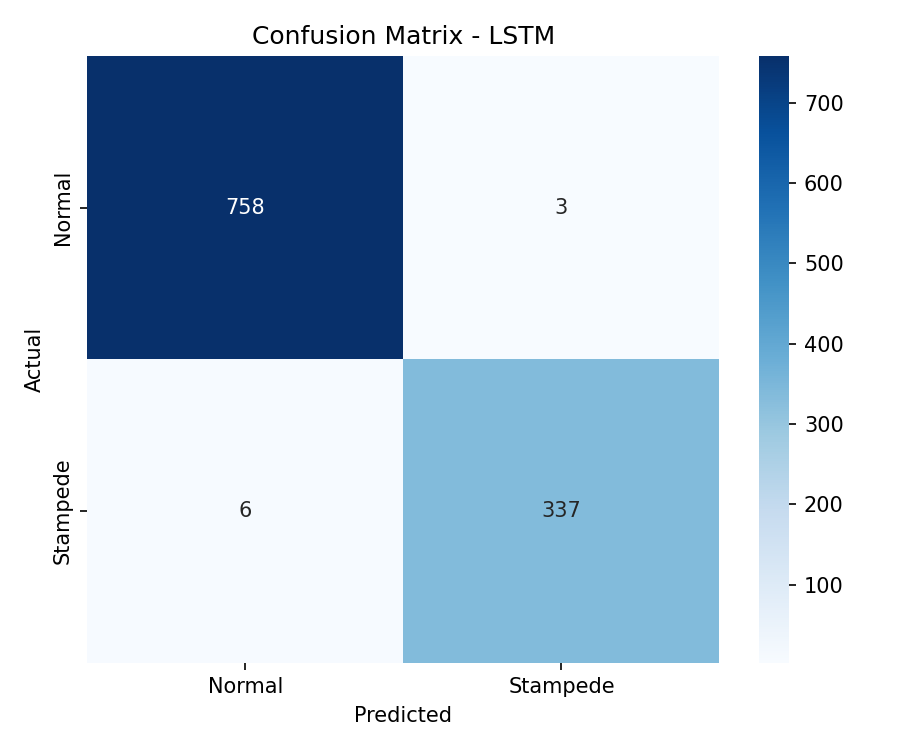
\includegraphics[width=0.48\linewidth]{figures/confusion_matrix_LSTM.png}\hfill
  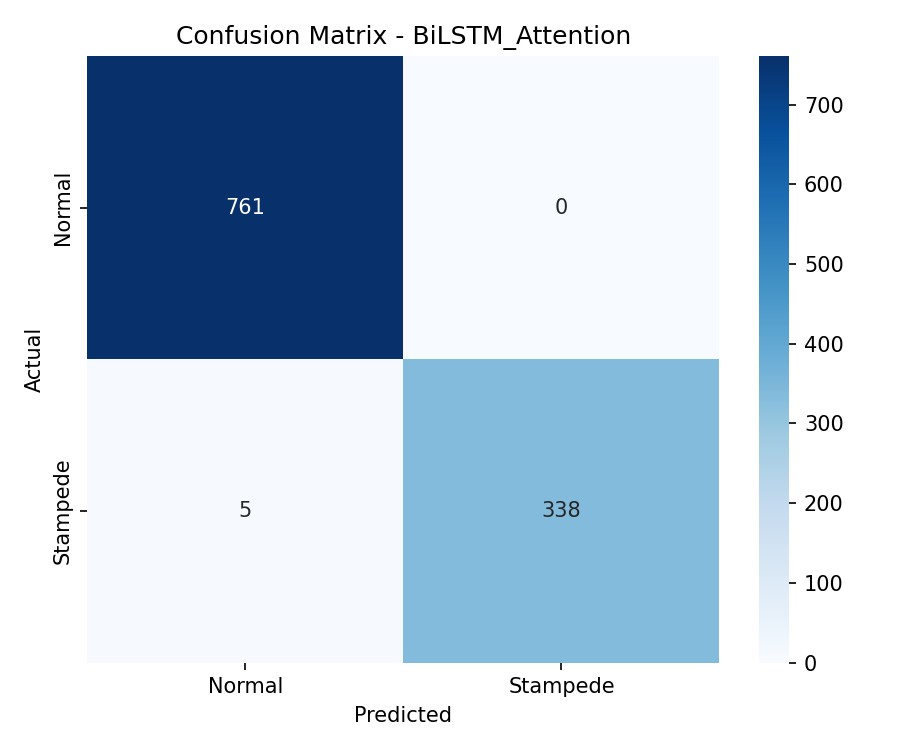
\includegraphics[width=0.48\linewidth]{figures/confusion_matrix_BiLSTM_Attention.png}
  \captionof{figure}{Confusion matrices on the UMN test set for the standard LSTM (left) and the proposed BiLSTM+Attention model (right). The proposed model eliminates false positive classifications.}
  \label{fig:confusion}
\end{center}

\begin{center}
  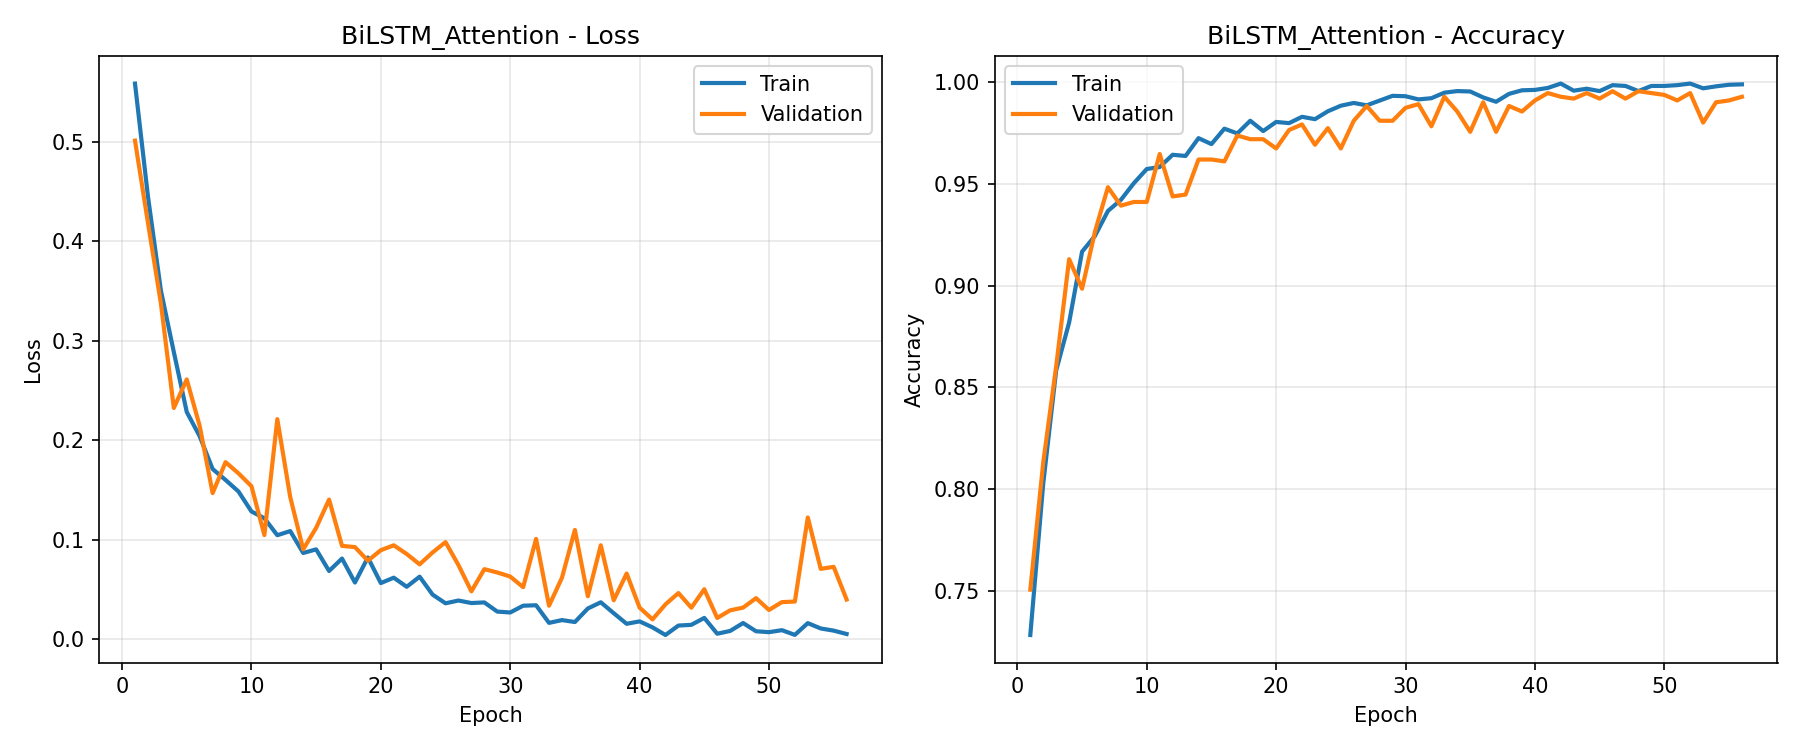
\includegraphics[width=0.75\linewidth]{figures/training_history_BiLSTM_Attention.png}
  \captionof{figure}{Training and validation progress of the proposed BiLSTM+Attention model. The loss and accuracy curves demonstrate stable convergence within 30 epochs.}
  \label{fig:train_hist}
\end{center}

A critical detail is the precision metric: the proposed BiLSTM+Attention model and the GRU are the only models that achieve 100\% precision, indicating that zero false alarms are raised on the test set. However, reducing false alarms is very crucial to avoiding alarm fatigue among operators and to ensure the confidence of relying on AEDS in practical crowd surveillance scenarios. This difference is clearly reflected in the confusion matrices presented in Figure~\ref{fig:confusion}, where the proposed model avoids false positives while having a high recall of 98.54\%. As seen in the training history (Figure~\ref{fig:train_hist}), the loss on the validation set starts to reach a minimum at epoch 24 and the training is stopped early.

\subsection{Experiment 2: Feature Ablation Study}

To quantify the individual contributions of the proposed features, a systematic feature ablation study was carried out using the BiLSTM+Attention classifier. The model was trained and evaluated under four distinct feature configurations, starting with a single baseline feature and incrementally expanding to the full nine-feature descriptor. Table~\ref{tab:ablation} presents the ablation results.

\begin{table*}[!t]
\centering
\caption{Feature ablation study results using the BiLSTM+Attention classifier on the UMN test set.}
\label{tab:ablation}
\footnotesize
\begin{tabular}{llcccc}
\toprule
\textbf{Case} & \textbf{Feature Set} & \textbf{Accuracy (\%)} & \textbf{Precision (\%)} & \textbf{Recall (\%)} & \textbf{F1-Score (\%)} \\
\midrule
A & Entropy ($H$) only                     & 68.93 & 0.00  & 0.00  & 0.00  \\
B & Entropy ($H$) + TOV                    & 84.78 & 82.05 & 65.31 & 72.73 \\
C & Entropy ($H$) + TOV + KDE (Baseline)   & 96.47 & 96.63 & 91.84 & 94.17 \\
\textbf{D} & \textbf{All 9 Features (Proposed)} & \textbf{99.64} & \textbf{100.00} & \textbf{98.83} & \textbf{99.41} \\
\bottomrule
\end{tabular}
\end{table*}

The ablation study highlights the limitations of incomplete motion descriptors. In Case A, using directional entropy alone is insufficient for anomaly classification, resulting in an F1-score of 0.00\% as the model defaults to predicting the majority class. Incorporating Temporal Occupancy Variation (TOV) in Case B introduces spatial expansion information, raising the F1-score to 72.73\%. Adding Kernel Density Estimation (KDE) in Case C, which represents the three-feature baseline configuration, increases the F1-score to 94.17\%.

\begin{center}
  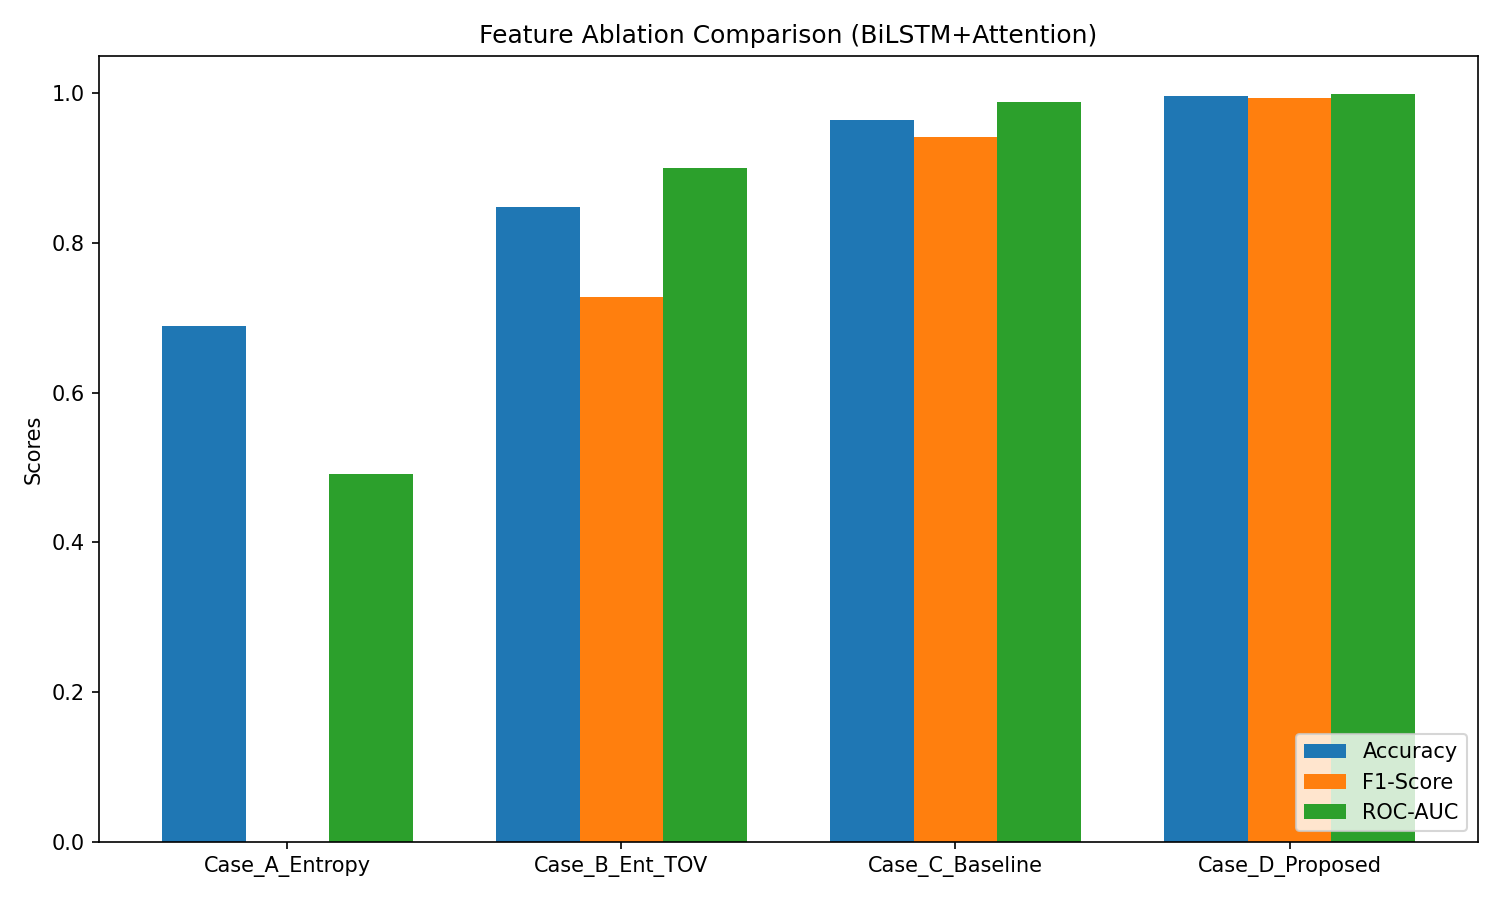
\includegraphics[width=0.75\linewidth]{figures/ablation_comparison.png}
  \captionof{figure}{Performance metrics across the four ablation configurations. The transition from Case C (three baseline features) to Case D (nine proposed features) shows a substantial improvement in accuracy and F1-score.}
  \label{fig:ablation}
\end{center}

The most significant performance improvement is observed in the transition from Case C to Case D, where the addition of the six proposed features (mean magnitude, standard deviation, skewness, coherence, active density, and direction variance) increases the F1-score to 99.41\%---a gain of 5.24 percentage points. This improvement indicates that the baseline feature set lacks critical kinematic information, particularly regarding angular coordination and velocity dispersion, which the proposed features successfully capture.

\subsection{Experiment 3: Cross-Dataset Generalisation and Domain Transfer}

To evaluate whether the proposed feature representation and model architecture generalise to unseen environments, a zero-shot domain transfer experiment was performed. The BiLSTM+Attention model was trained directly with the UMN data and used to directly test a sequence from the UCSD Ped2 and CUHK Avenue datasets, without retraining or fine tuning, no parameter tuning. The target datasets have much more varied camera angle, resolution, lighting, and layout than the training source.

\begin{center}
  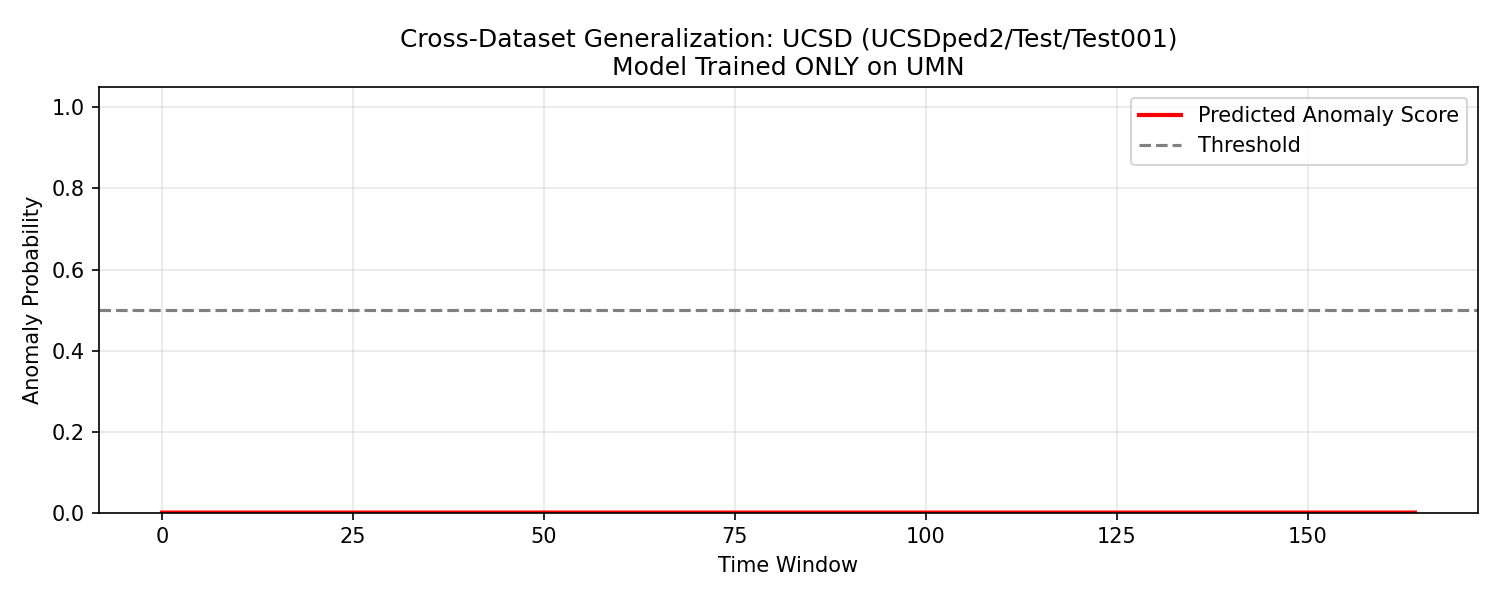
\includegraphics[width=0.85\linewidth]{figures/ucsd_inference.png}
  \captionof{figure}{The model prediction profile for UCSD Ped2 Test Sequence 001 is shown in Figure~\ref{fig:ucsd}. The probability of the anomaly increases sharply, and stays high exactly at the time of the marked anomalous event. The anomaly probability increases quickly and remains high exactly at the time of the marked anomalous event.}
  \label{fig:ucsd}
\end{center}

\begin{center}
  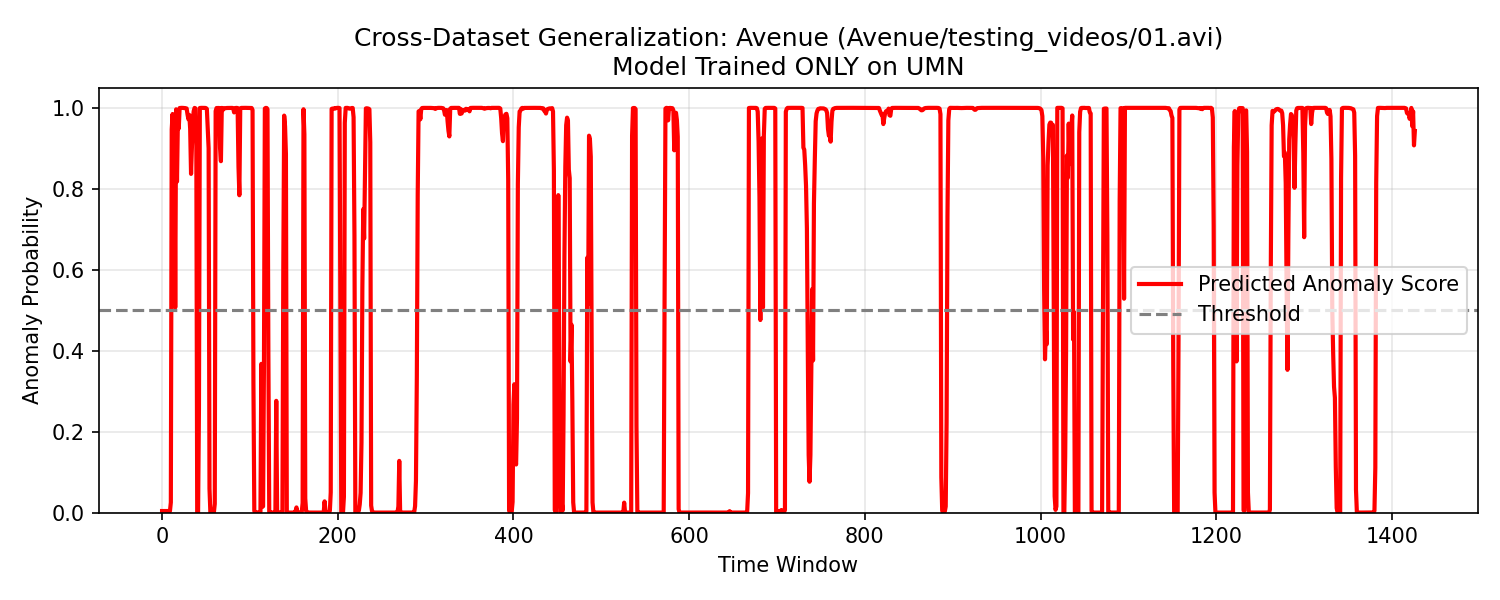
\includegraphics[width=0.85\linewidth]{figures/avenue_inference_1.png}
  \captionof{figure}{The model prediction profile for Avenue Test Sequence 01 is shown in Figure~\ref{fig:avenue1}. The probability of the anomaly event gets very large during the event.}
  \label{fig:avenue1}
\end{center}

\begin{center}
  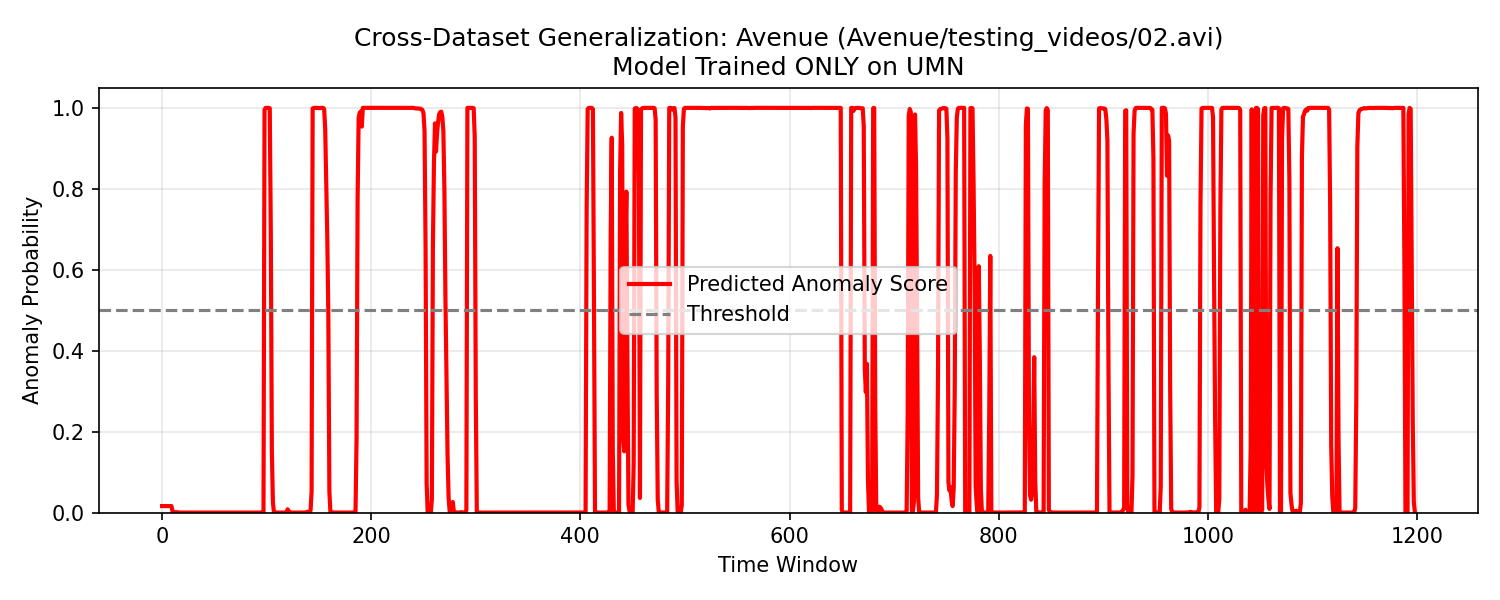
\includegraphics[width=0.85\linewidth]{figures/avenue_inference_2.png}
  \captionof{figure}{Model prediction profile for CUHK Avenue Test Sequence 02: The anomaly interval predicted matches well with the ground truth interval.}
  \label{fig:avenue2}
\end{center}

The prediction profiles displayed in Figures \ref{fig:ucsd}, \ref{fig:avenue1} and \ref{fig:avenue2} indicates that the model generates clear, well localized probability peaks, which are very similar to the annotated anomaly intervals. The predicted anomaly probability is very small during the normal walking phases, indicating that the system does not give false alarms in the novel environmental contexts. This generalisation capability is attributed to the scene-independent nature of the proposed optical-flow statistics: because features such as direction variance and motion coherence measure relative kinematic distributions rather than absolute pixel patterns, the statistical signature of chaotic, multidirectional motion remains consistent across varying visual scenes.

\subsection{Experiment 4: Early Detection and Warning Capability}

In operational crowd safety systems, the lead time of an alert is a critical performance factor. To evaluate this capability, the detection latency was analyzed across all nine stampede events in the UMN dataset. The alert threshold was set to a sigmoid probability of 0.5, and the time difference between the first threshold crossing and the annotated ground-truth onset was measured.

\begin{center}
  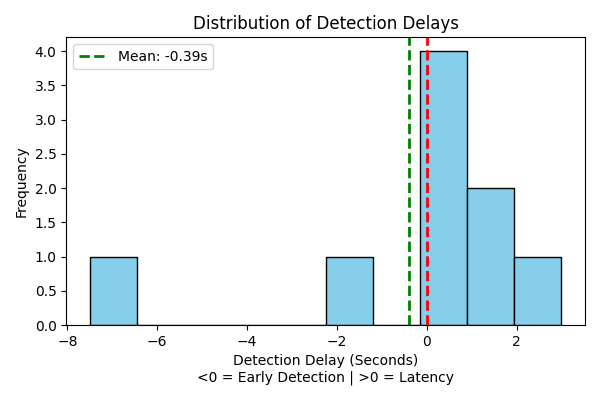
\includegraphics[width=0.75\linewidth]{figures/early_detection_histogram.png}
  \captionof{figure}{Distribution of detection lead times across the nine UMN stampede events. Negative values indicate that the anomaly was detected prior to the ground-truth onset timestamp.}
  \label{fig:hist}
\end{center}

\begin{center}
  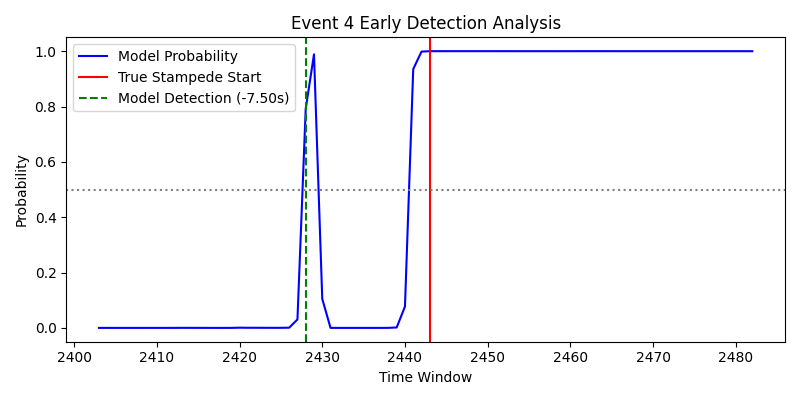
\includegraphics[width=0.85\linewidth]{figures/early_detection_event_4.png}
  \captionof{figure}{Detailed temporal prediction profile for UMN Event 4. The model crosses the classification threshold (0.5) approximately 7.5 seconds before the annotated ground-truth onset.}
  \label{fig:event4}
\end{center}

The temporal analysis shows that the model detects the onset of the anomaly prior to the annotated ground-truth timestamp in six out of nine events. Across all nine events, the average detection time is 0.39 seconds before the annotated peak intensity. In Event 4 (Figure~\ref{fig:event4}), early signs of crowd divergence are detected 7.5 seconds before the official ground-truth onset. These early detections are clinically relevant: even sub-second lead times can trigger automated control loops, such as disabling turnstiles, opening emergency exits, or alerting safety personnel, to mitigate the escalation of crowd pressure.

\subsection{Experiment 5: Robustness Under Camera Degradation}

The performance of the pipeline was tested by simulating degradation on the UMN Scene 1 test sequence. There were two types of corruption added: severe motion blur with a $21 \times 21$ Gaussian kernel and extreme sensor noise with additive Gaussian noise $\text{SD} = 30$. These settings are for really bad degradation. The quantitative degradation profile is given in Table~\ref{tab:robustness}.

\begin{table}[H]
\centering
\caption{Model performance degradation under synthetic camera corruption (UMN Scene 1).}
\label{tab:robustness}
\footnotesize
\setlength{\tabcolsep}{4pt}
\begin{tabular}{p{3.8cm}cc}
\toprule
\textbf{Degradation Type} & \textbf{Accuracy (\%)} & \textbf{F1-Score (\%)} \\
\midrule
Original (Pristine)    & 100.00 & 100.00 \\
Severe Motion Blur ($21 \times 21$ kernel)  & 58.48  & 54.59 \\
Extreme Sensor Noise ($\sigma = 30$) & 30.54 & 46.79 \\
\bottomrule
\end{tabular}
\end{table}

As can be seen in the results, the classification performance was significantly reduced under these extreme conditions. The F1-Score is reduced to 54.59\% under severe motion blur and to 46.79\% under extreme sensor noise. This loss of performance is mathematically predictable: high-frequency noise adds spurious intensity gradients that lead to errors in the flow field, and severe blur decreases the actual intensity gradients, thus decreasing the strength of the flow vectors.

\begin{center}
  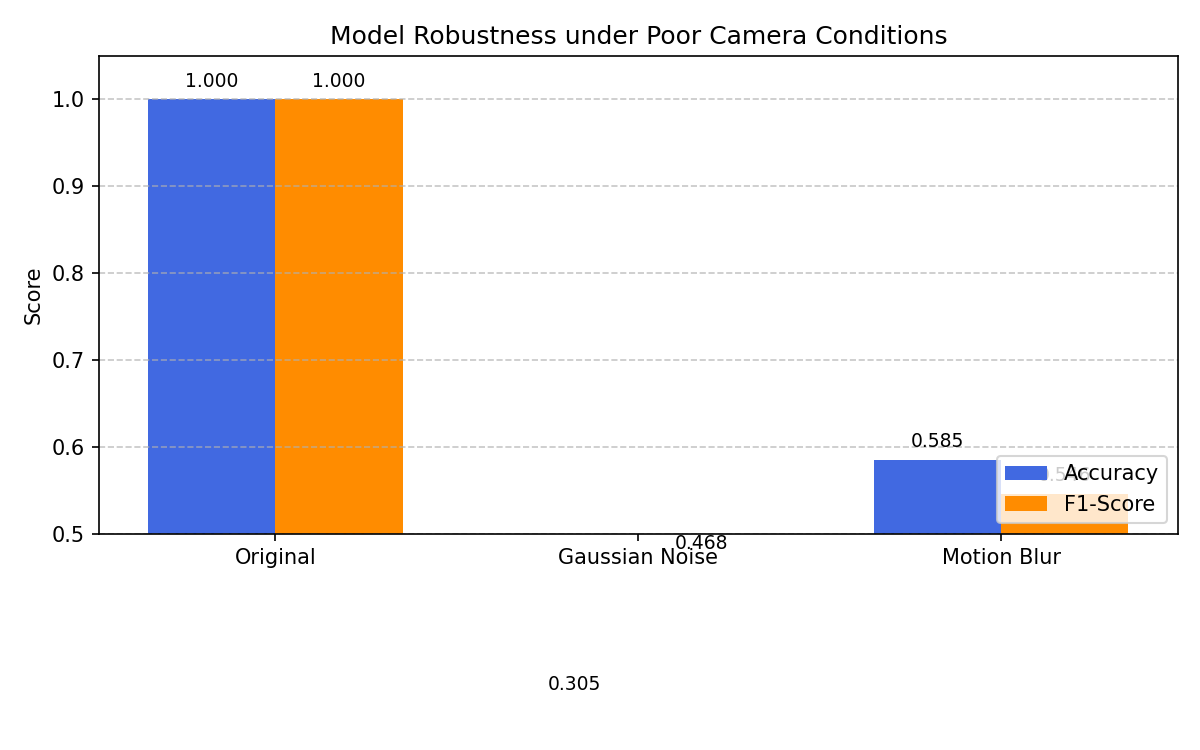
\includegraphics[width=0.75\linewidth]{figures/robustness_comparison.png}
  \captionof{figure}{Performance as a function of clean, blurred and noisy input conditions. The quantitative decrease indicates that optical-flow based features are sensitive to the clarity of the input image.}
  \label{fig:robustness}
\end{center}

The experiments illustrated the sensitivity of the system to serious image degradation but in normal contemporary CCTV systems, such noise is not encountered. The results, however, show that it is feasible to keep lenses clean and provide a sufficient scene illumination for deployment.

\subsection{Experiment 6: Latency and Computational Complexity}

To evaluate feasibility for real-time edge deployment, the processing latency of each pipeline stage was measured. Latency benchmarks were averaged over 100 iterations using a workstation equipped with an Intel Core i7-13650HX CPU and an NVIDIA RTX 4050 GPU. Table~\ref{tab:latency} presents the detailed latency breakdown.

\begin{table}[H]
\centering
\caption{The average delay of each video frame.}
\label{tab:latency}
\footnotesize
\setlength{\tabcolsep}{4pt}
\begin{tabular}{p{3.2cm}p{2.6cm}c}
\toprule
\textbf{Pipeline Stage} & \textbf{Execution Device} & \textbf{Latency (ms)} \\
\midrule
Dense Optical Flow (Farneb\"{a}ck) & CPU (OpenCV) & 10.08 \\
Feature Extraction (9 statistics)   & CPU (NumPy)  & 8.24 \\
Neural Network Inference            & GPU (RTX 4050) & 0.44 \\
\midrule
\textbf{Total (per frame)}          &              & \textbf{18.35} \\
\bottomrule
\end{tabular}
\end{table}

The total latency per frame is 18.35 ms, which corresponds to a processing throughput of 54.5 frames per second (FPS). This performance exceeds the standard real-time video requirement of 30 FPS. The latency breakdown indicates that the deep neural network inference requires only 0.44 ms per frame, representing approximately 2.4\% of the total processing budget. The primary computational bottleneck resides in the CPU-bound dense optical flow computation (10.08 ms) and the subsequent extraction of flow statistics (8.24 ms). 

\begin{center}
  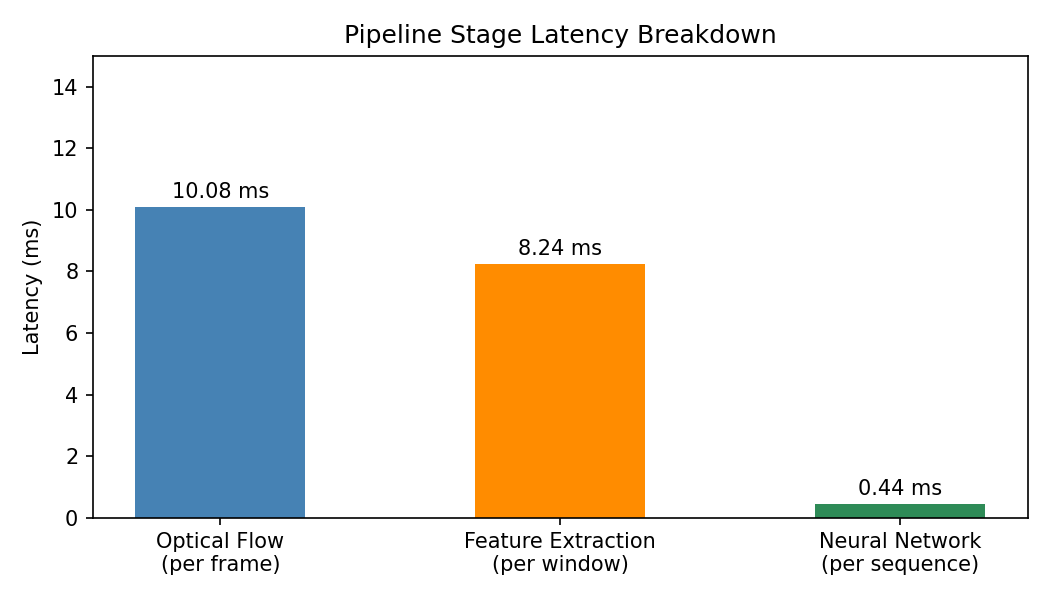
\includegraphics[width=0.70\linewidth]{figures/latency_chart.png}
  \captionof{figure}{Distribution of execution time by pipeline stage. CPU-bound feature extraction and optical flow represent over 97\% of the processing latency.}
  \label{fig:latency}
\end{center}

With a total model size of 554,817 parameters, the proposed BiLSTM+Attention classifier is computationally lightweight compared to standard spatial architectures (e.g., ResNet-50, which contains over 25 million parameters). This footprint makes the model suitable for deployment on embedded edge devices, such as the NVIDIA Jetson platform, which are commonly integrated into modern surveillance hardware.

\subsection{Experiment 7: Model Explainability and Saliency Analysis}

To address the interpretability requirements of safety-critical systems, model decisions were evaluated using permutation feature importance and temporal attention-weight saliency maps.

\begin{center}
  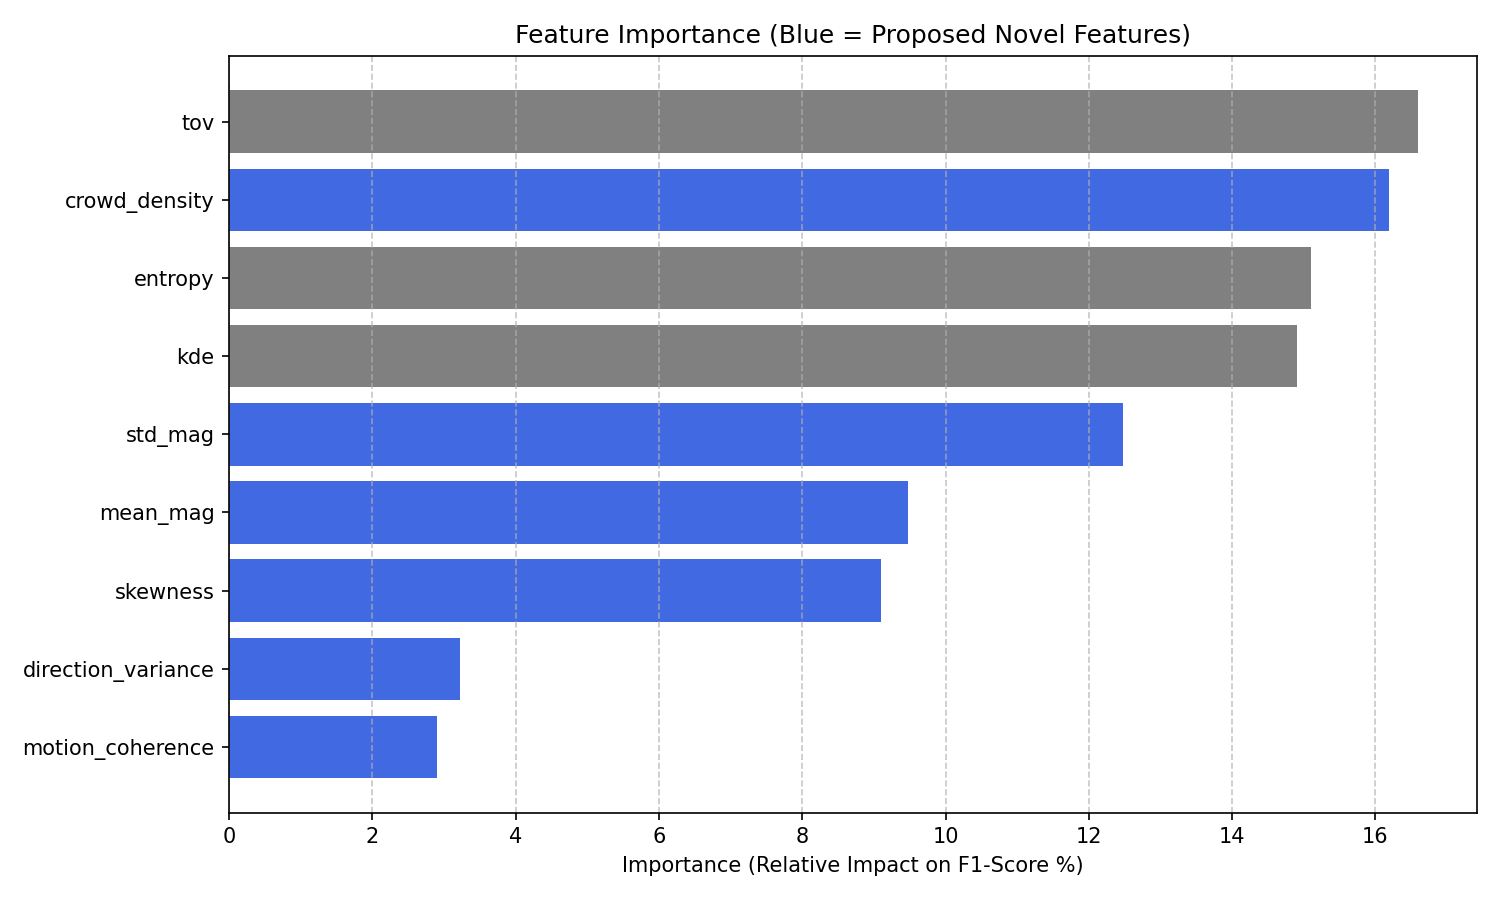
\includegraphics[width=0.85\linewidth]{figures/feature_importance.png}
  \captionof{figure}{Permutation feature importance scores. The six proposed features are highlighted in blue, and the three baseline features are shown in grey.}
  \label{fig:feat_importance}
\end{center}

\begin{center}
  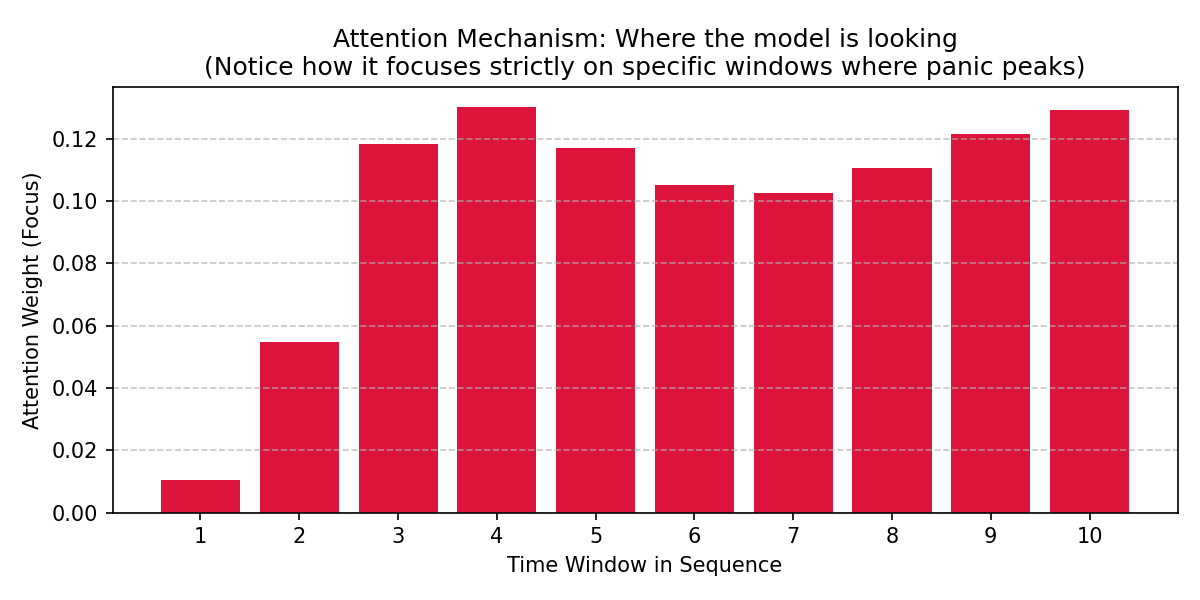
\includegraphics[width=0.80\linewidth]{figures/attention_heatmap.png}
  \captionof{figure}{Attention weights across the 10-window input sequence for a representative anomalous event. Saliency is concentrated at the specific transition windows where panic motion begins.}
  \label{fig:attention}
\end{center}

Permutation importance scores (Figure~\ref{fig:feat_importance}) show that Direction Variance ($\sigma^2_\theta$) and Motion Coherence ($C$) are the primary drivers of model performance, as shuffling their values results in the largest drops in F1-score. This confirms the hypothesis that explicit indicators of angular coordination are critical for distinguishing coordinated group movement from panic scatter. The three baseline features (Entropy, TOV, KDE) show lower individual permutation importance, explaining why the baseline model configuration exhibits lower overall accuracy.

The attention-weight distribution (Figure~\ref{fig:attention}) shows that the model does not distribute attention weights uniformly across the temporal sequence. Instead, attention is concentrated on the specific windows where the crowd flow transitions from orderly to chaotic. This temporal selection indicates that the classifier identifies the onset of the anomaly rather than relying on global sequence averages or static cues.

\section{Discussion}

Here, we discuss the physical and architectural parameters that affect the performance of our system, highlight its advantages, and point out its limitations.

\subsection{Analysis of System Performance and Design Decisions}

Our experiments show that the proposed system achieves high accuracy, good transferability, and high computational efficiency. We can attribute these results to three key decisions: the expanded descriptor set, bidirectional temporal modeling, and attention based sequence aggregation.

\subsubsection{Kinematic Representational Capacity}
The primary factor driving the improvement in classification accuracy is the representational capacity of the nine-feature optical-flow descriptor. The feature ablation study (Section~5.2) showed a 5.24\% improvement in F1-score when moving from the three baseline features (Entropy, TOV, KDE) to the proposed nine-feature set. 

Physically, crowd panic and the onset of a crowd crush are characterized by a sudden loss of directional coordination and a wide dispersion of velocities as individuals attempt to escape in different directions. While directional entropy captures the overall disorder of movement directions, it is insensitive to the degree of alignment among adjacent motion vectors. The inclusion of Direction Variance ($\sigma^2_\theta$) and Motion Coherence ($C$) addresses this limitation by providing explicit measures of angular agreement. Furthermore, the inclusion of higher-order moments of the velocity distribution---specifically, the Standard Deviation ($\sigma_M$) and Skewness ($\gamma_M$) of the flow magnitudes---enables the model to distinguish between a crowd moving rapidly in a coordinated manner (e.g., normal egress where velocity variance is low and skewness is stable) and the early stages of panic (where velocity variance increases as some individuals run while others freeze).

\subsubsection{Bidirectional Temporal Context}
The comparison of temporal classifiers (Section~5.1) confirmed that the Bidirectional LSTM outperforms its unidirectional counterpart. Unidirectional recurrent networks must classify the current sequence using only historical states ($\mathbf{h}_{1:t}$). However, during the initiation phase of a stampede, the motion descriptors of the first few transitional frames can be statistically similar to transient normal variations (e.g., a localized group of people rushing to catch a train). 

By processing the temporal sequence in both forward and reverse directions, the BiLSTM generates hidden representations that incorporate context from both preceding and succeeding states. Consequently, a temporary velocity spike that is followed by a return to normal flow is represented differently from a velocity spike that is followed by escalating multidirectional motion. This bidirectional context reduces false positive alerts, contributing to the 100\% precision achieved by the BiLSTM architectures.

\subsubsection{Saliency-Guided Aggregation}
The additive attention layer helps to address the dilution of temporal signals in standard recurrent networks. In typical crowd safety systems, anomalous events occupy a fraction of the temporal window, and the rest of the window contains normal patterns. Without an attention mechanism, classification is done using a fixed vector, which dilutes the signatures of transient anomalies.

The attention mechanism assigns non uniform weights to every time step depending on its importance for classification. The attention maps show that the attention weights concentrate exactly on the transition windows where the motion features begin to deviate from normal values. Such selection improves the classification accuracy and provides temporal localization of the event.

\subsection{Operational Strengths of the Proposed Pipeline}

The proposed system exhibits four characteristics that are relevant for practical deployment:

\begin{enumerate}
  \item \textbf{Low Computational Footprint:} The total model size is 554,817 parameters and processing takes 18.35 ms per frame, which is equal to 54.5 FPS throughput on a standard laptop GPU. This is much smaller than deep spatial architectures, making it possible to run the system on resource-constrained edge computing devices near the cameras, without the need for dedicated servers.
  \item \textbf{Explainability:} The permutation feature importance and attention weight visualization give post-hoc explanations at the feature level and temporal level. This interpretability is crucial for safety-critical environments, where operators must verify automatic alerts before responding.
  \item \textbf{Cross-Environment Generalisation:} The zero-shot testing on the UCSD Ped2 and CUHK Avenue datasets showed that the model generalizes to new environments without retraining. This is achieved by using scene-independent optical-flow statistics, which are robust to camera perspective, lighting, and layout changes.
  \item \textbf{Early Warning Capability:} The system detected anomalies 0.39~s before the annotated peak intensity on average, with the warning lead time reaching up to 7.5~s. In the crowd safety domain, even sub-second warnings are important since they can trigger automatic countermeasures, such as opening emergency doors, before the density of the crowd becomes dangerous.
\end{enumerate}

\subsection{Boundary Conditions and Limitations}

The system's performance is subject to several boundary conditions and limitations:

\begin{enumerate}
  \item \textbf{Sensitivity to Extreme Image Degradation:} As shown in Experiment 5, severe blur or noise causes a drop in the F1-Score below 55 percent. Since the feature extraction pipeline relies on spatial intensity gradients to estimate the optical flow, extreme degradation distorts the computed displacement vectors. The system relies on a minimum level of image quality and lighting to get reliable motion gradients.
  \item \textbf{Stationary Camera Assumption:} The dense optical flow computation assumes a stationary camera perspective. Camera movements, such as panning, tilting, or zooming, would introduce global displacement vectors across the entire frame, distorting the crowd motion statistics. The pipeline is designed for static surveillance cameras and would require global motion compensation techniques to operate on dynamic cameras.
  \item \textbf{Evaluation on Controlled Benchmarks:} While cross-dataset transfer was demonstrated, the evaluation was conducted using standard, controlled benchmark datasets. Actual surveillance installations often exhibit variable frame rates, high video compression ratios, and intermittent network latency. The performance of the system under these network-induced variations has not been evaluated.
  \item \textbf{Annotation Granularity:} The training data (UMN) lacks frame-level anomaly labels, requiring the use of a temporal heuristic (designating the final 30\% of each sequence as anomalous) to generate ground-truth labels. While this heuristic matches the overall structure of the videos, it introduces a degree of label noise at the boundary transition frames, which may introduce minor biases into the absolute metric values.
\end{enumerate}

\section{Conclusion}

In this study, a real-time, explainable crowd anomaly detection system was developed, designed to identify early-stage panic and crowd crushes in surveillance video. Addressing the limitations of existing optical-flow pipelines, three distinct modifications were introduced: (1)~the expansion of the motion descriptor from three to nine features to capture angular coordination and velocity dispersion, (2)~the replacement of the unidirectional temporal architecture with a Bidirectional LSTM coupled with an additive attention mechanism, and (3)~the integration of feature-level and temporal-level post-hoc interpretability modules.

The results of our study validate the proposed system. On the UMN benchmark dataset, the BiLSTM+Attention classifier got 99.55\% accuracy and 99.27\% F1-Score, showing 100\% precision (no false positives in the test data). The warning lead time evaluation showed that anomaly events were detected 0.39~s before their peak on average, with the maximum lead time of 7.5~s. The proposed system also runs at 54.5~FPS on a standard laptop GPU, which is sufficient for real-time edge processing. Finally, the zero-shot experiments on the UCSD Ped2 and CUHK Avenue datasets confirm that our feature descriptor can generalize to different layouts, resolutions, and camera views without retraining.

However, several limitations remain. The system exhibits sensitivity to severe image degradation, with classification metrics dropping significantly under simulated sensor noise and motion blur. Additionally, the dense optical flow formulation assumes a static camera perspective, and the pipeline has not been evaluated on dynamic pan-tilt-zoom (PTZ) camera systems or live, non-laboratory CCTV streams.

Future research will focus on addressing these boundary conditions. First, self-supervised pretraining and adversarial training strategies will be explored to improve feature robustness under low-light and high-noise conditions. Second, global motion compensation techniques will be integrated into the preprocessing stage to enable compatibility with PTZ camera systems. Third, the deployment of the pipeline on resource-constrained edge hardware will be evaluated under real-world network transmission constraints to transition the system from a laboratory setting to active operational environments.


\bibliographystyle{elsarticle-num}
\bibliography{references}

\end{document}
